%  LaTeX support: latex@mdpi.com 
%=================================================================
\documentclass[agriculture,article,submit,pdftex,moreauthors]{Definitions/mdpi} 

%=================================================================
\firstpage{1} 
\makeatletter 
\setcounter{page}{\@firstpage} 
\makeatother
\pubvolume{1}
\issuenum{1}
\articlenumber{0}
\pubyear{2026}
\copyrightyear{2026}
\datereceived{ } 
\daterevised{ } 
\dateaccepted{ } 
\datepublished{ } 
\setlength{\headheight}{20pt}

\usepackage{booktabs}
\usepackage{graphicx}
\graphicspath{{figures/}}

%=================================================================
\Title{Regime-Dependent Performance of Generic CLIP Representations for Fine-Grained Tobacco Disease Classification}

\Author{Lizhuo Li $^{1,}$*}

\AuthorNames{Lizhuo Li}

\address{%
$^{1}$ \quad School of Information Science and Engineering, Yunnan University, Kunming 650091, China; lizhuo@ynu.edu.cn}

\corres{Correspondence: lizhuo@ynu.edu.cn}

\simplesumm{This single-crop (tobacco), single-dataset study examines whether the widely used CLIP vision-language model can classify fine-grained tobacco leaf disorders without any domain-specific training. It cannot do so zero-shot, but with a small amount of domain data its frozen features reach roughly the same overall accuracy as a fine-tuned small CNN (within a few percentage points; under 5-fold cross-validation the CNN holds a small, stable edge of about 4 percentage points, sign-stable across all five folds), even as the CNN remains the more robust option on the rare, fine-grained classes (on this test set, a difference driven mainly by a handful of single-image classes).}

%=================================================================
\abstract{%
Whether widely used vision-language models (VLMs) such as CLIP can classify fine-grained plant diseases without domain-specific training is a practical question for resource-constrained settings. We address it for \emph{tobacco} leaf disorders, and---to test whether the conclusion is tobacco-specific---replicate the full protocol on a \emph{second crop} (tomato).
We compare two generic CLIP variants (DFN-CLIP and LAION-2B, both ViT-L/14, 428M parameters) against a fine-tuned ResNet-18 (12M parameters) on a primary 16-class dataset (TPDD) across zero-shot, few-shot, and full-data regimes, with the zero-shot result cross-checked on an external 10-class dataset (TLD) and the full protocol replicated cross-crop on a 10-class tomato dataset (PlantVillage).
\textbf{Zero-shot CLIP fails.} On both datasets the best of 14 templates sits at or below the majority-class baseline (TPDD 13.0\% vs.\ a 13.0\% baseline; TLD 17.7\% vs.\ a 19.0\% baseline), and no template, including KG-augmented ones, yields a reliable gain.
\textbf{With minimal domain data the outcome is regime-dependent.} At $K{=}1$ (seed-paired support sets) the LAION-2B probe is higher than fine-tuned ResNet-18 (38.5\% vs.\ 32.1\%; $+6.4$ percentage points (pp), $p=0.0003$) while the DFN-CLIP probe trails by 3.7\,pp; this $K{=}1$ lead is partly a probe-protocol effect, since a frozen ResNet-18 linear probe on the same support sets already reaches 34.1\%, above the fine-tuned 32.1\%, and is checkpoint-specific (LAION-2B leads while DFN-CLIP trails). At $K{=}5$--$10$ the fine-tuned ResNet-18 is higher for both CLIP probes (5.6--17.6\,pp).
 \textbf{At full data the two are close on top-1 accuracy, with a small, stable CNN edge under proper resampling.} On the held-out 138-image split a validation-regularized CLIP probe reaches 85.5\% (LAION-2B 86.2\%), within $\approx$1\,pp of fine-tuned ResNet-18 (86.4\%); under 5-fold cross-validation over the training pool, fine-tuned ResNet-18 leads the frozen CLIP probe by a small, sign-stable margin ($87.8\%$ vs.\ $92.1\%$; $-4.3\,\text{pp}\pm1.8$, all five folds). This is a close, split-dependent comparison---descriptive, not an equivalence claim, and not resolvable at the per-image level (per-image standard error $\approx$3.4\,pp). The balanced-accuracy gap (77.4\% vs.\ 84.3\%) is driven largely by the rare (singleton) test classes, with a smaller contribution from a mid-frequency class.
 \textbf{The pattern is not tobacco-specific.} Replicated in full on a 10-class tomato set (PlantVillage, 18{,}160 images), zero-shot CLIP again sits at the majority baseline (33.4\% vs.\ 29.5\%), the frozen CLIP probe is competitive at $K{=}1$ (44.7\% vs.\ 40.4\% fine-tuned ResNet-18) while ResNet-18 leads at $K{=}5$--$10$ (73.6\% and 84.4\%), and full-data near-parity holds with a small, sign-stable CNN edge under 5-fold cross-validation (CLIP 98.0\% vs.\ 99.5\%; $-1.6\,\text{pp}$, all five folds)---the same regime-by-regime ordering as tobacco.
The zero-shot failure is consistent with a text--image decision-rule mismatch: the same frozen features reach 85.5\% under a supervised probe. In short, generic off-the-shelf CLIP is unreliable for zero-shot fine-grained tobacco-lesion classification, but with minimal domain training its frozen features are a checkpoint-specific, training-light baseline at low data (an advantage that is partly a probe-protocol artifact) and reach a descriptive, per-image-unresolvable near-parity with a fine-tuned CNN at full data; the CNN remains the more robust and cheaper-to-deploy option on the rare, fine-grained classes.
}

\keyword{CLIP; zero-shot classification; agricultural disease diagnosis; vision-language models; few-shot learning; knowledge graph; prompt engineering}

%%%%%%%%%%%%%%%%%%%%%%%%%%%%%%%%%%%%%%%%%%
\begin{document}

%%%%%%%%%%%%%%%%%%%%%%%%%%%%%%%%%%%%%%%%%%
\section{Introduction}
\label{sec:intro}

Vision-language models (VLMs) pretrained on web-scale image-text pairs, such as CLIP~\cite{radford2021learning}, have achieved strong zero-shot generalization across general-purpose visual recognition benchmarks.
This has led to growing enthusiasm for applying VLMs to specialized domains---including agriculture~\cite{pdclip2026}, medicine~\cite{huang2021gloria}, and remote sensing~\cite{liu2024remoteclip}---under the implicit assumption that large-scale pretraining transfers without additional training.

However, the visual statistics of specialized domains differ fundamentally from general web images.
Agricultural disease images feature fine-grained, domain-specific patterns (e.g., leaf lesions, fungal mycelia, chlorosis) that may be underrepresented in web-scale training corpora.
Whether and to what extent generic VLMs recognize these patterns remains an open empirical question with significant practical implications: if VLMs fail, practitioners would be misled; if they succeed, annotation costs could be reduced.

Recent work has explored domain-specific VLM adaptations. SCOLD~\cite{scold2025} pretrains a vision-language foundation model on over 186,000 leaf image-caption pairs, while BioCLIP 2~\cite{bioclip2} shows that 214M organism-image contrastive pretraining yields emergent zero-shot abilities on biological tasks. LP++~\cite{lpplus} proposes a learnable image-text knowledge blending linear probe that significantly surpasses naive CLIP probing. These adaptations require large-scale domain-specific pretraining; we empirically evaluate one such model, BioCLIP 2, as a domain-VLM control in the zero-shot results below and find it likewise sits at the majority-class baseline.

In contrast, off-the-shelf CLIP is evaluated without agricultural fine-tuning---a question of immediate relevance for practitioners lacking resources for domain-specific pretraining. This work provides an empirical boundary for off-the-shelf CLIP's applicability in resource-constrained settings, systematically comparing against ResNet-18 across data regimes and testing whether KG-augmented prompts can mitigate the lack of domain adaptation. Our core contribution is a within-crop boundary for off-the-shelf CLIP on tobacco; to test whether the regime-by-regime pattern is crop-specific or more general, we additionally replicate the full protocol on a second crop (tomato, PlantVillage) under the identical split, probe, and evaluation conditions.

This investigation is guided by three research questions:

\begin{itemize}
    \item \textbf{RQ1.} Can CLIP zero-shot classify tobacco diseases, and do KG-augmented prompts help?
    \item \textbf{RQ2.} How does CLIP linear probe compare to end-to-end ResNet-18 across data regimes?
    \item \textbf{RQ3.} Do the zero-shot / few-shot / full-data model rankings generalize across crops (tomato PlantVillage in addition to tobacco TPDD and TLD)?
\end{itemize}

Four main findings are reported:
(1) Zero-shot CLIP shows no detectable improvement over the trivial majority-class baseline for fine-grained tobacco lesions: the best of 14 templates (13.0\%) matches always-predicting-the-common-class (13.0\%), no top-performing template's confidence interval excludes this baseline, and KG-augmented prompts show no reliable gain over plain captions under the experimental conditions.
(2) The CLIP--ResNet comparison is regime-dependent: the LAION-2B CLIP probe attains a higher accuracy than ResNet-18 at $K{=}1$ (38.5\% vs.\ 32.1\%; seed-paired support sets, $+6.4$\,pp, $p=0.0003$) while the DFN-CLIP variant trails by 3.7\,pp, at $K{=}5$--$10$ the fine-tuned ResNet leads both CLIP probes, and at full data a validation-regularized probe reaches 85.5\% (LAION-2B 86.2\%), within $\approx$1\,pp of fine-tuned ResNet-18 on top-1 accuracy (a descriptive gap; no equivalence claim), with 5-fold cross-validation showing fine-tuned ResNet-18 holding a small, sign-stable edge ($87.8\%$ vs.\ $92.1\%$, $\approx$4\,pp)---the default un-regularized probe trails ResNet (76.8\% vs.\ 86.4\%), and on balanced accuracy ResNet holds a substantial edge (84.3\% vs.\ 77.4\%), a metric sensitive to the four singleton test classes, surfacing a minority-class deficit that top-1 accuracy masks.
(3) The at-baseline zero-shot failure also holds on the external TLD set (best 17.7\%, descriptively below its 19.0\% majority baseline); this is consistent with a mismatch between the zero-shot text--image decision rule and the discriminative information in the frozen visual representation---the measured global feature-geometry metrics (inter/intra-class ratio 0.62 on the training split, 0.81 on the held-out split) do not indicate that poor visual separability alone explains the failure (the same features reach 85.5\% under a supervised probe).
(4) Replicating the full protocol on a second crop (tomato, PlantVillage, 18{,}160 images) reproduces the same regime-by-regime pattern---zero-shot at the majority baseline (33.4\% vs.\ 29.5\%), the frozen CLIP probe competitive at $K{=}1$ with fine-tuned ResNet-18 leading at $K{=}5$--$10$, and full-data near-parity with a small, sign-stable CNN edge under 5-fold CV ($98.0\%$ vs.\ $99.5\%$, $-1.6$\,pp)---indicating the finding is a property of off-the-shelf CLIP in fine-grained leaf-disease settings, not of tobacco specifically.

%%%%%%%%%%%%%%%%%%%%%%%%%%%%%%%%%%%%%%%%%%
\section{Related Work}
\label{sec:related}

\subsection{Vision-Language Models for Specialized Domains}

CLIP~\cite{radford2021learning} and its variants~\cite{zhai2023sigmoid,cherti2023reproducible} have enabled zero-shot image classification through natural language prompts, achieving strong results on standard benchmarks such as ImageNet~\cite{deng2009imagenet}, but systematic evaluation on small, imbalanced agricultural datasets remains limited.
Subsequent work has explored domain-specific adaptations such as BioCLIP~\cite{stevens2024bioclip} for organism classification and medical VLMs for radiology~\cite{huang2021gloria}, alongside agriculture-specific evaluation via the AgroBench vision-language benchmark~\cite{shinoda2025agrobench}.
In the leaf-disease domain specifically, SCOLD~\cite{scold2025} pretrains a vision-language foundation model on over 186,000 leaf image-caption pairs, and BioCLIP 2~\cite{bioclip2} shows that 214M organism-image contrastive pretraining yields emergent zero-shot abilities on biological tasks.
These adaptations require large-scale domain-specific pretraining.
In contrast, off-the-shelf CLIP is evaluated without agricultural fine-tuning---a question of immediate relevance for practitioners lacking resources for domain-specific pretraining.

\subsection{CLIP Prompt Engineering}

Prompt design significantly affects CLIP zero-shot performance~\cite{zhou2022learning,liu2025finegrained}, and domain-specific prompts have been reported to outperform generic ones in specialized settings.
Prior work has proposed prompt ensembling~\cite{radford2021learning}, learnable contexts~\cite{zhou2022learning}, and class-specific templates.
In agricultural domains, KGs encode structured disease information~\cite{cropdpkg2025}.
It is tested whether KG-derived symptom descriptions, a text-only pathway for injecting domain knowledge, can improve CLIP zero-shot classification.

\subsection{Few-Shot vs.\ Zero-Shot in Agriculture}

Few-shot learning has been studied for crop disease classification~\cite{argueso2020fewshot,liang2021cotton}, building on the large PlantVillage dataset~\cite{plantvillage2016} that established the standard benchmark for leaf-disease classification.
Systematic comparisons between zero-shot VLMs and few-shot domain models remain rare.
Agriculture-specific vision-language benchmarks such as AgroBench~\cite{shinoda2025agrobench} evaluate existing models on crop tasks but do not, in the surveyed literature, report controlled multi-seed replication of zero-shot results.
This work provides a statistically rigorous head-to-head comparison across two datasets.

%%%%%%%%%%%%%%%%%%%%%%%%%%%%%%%%%%%%%%%%%%
\section{Materials and Methods}
\label{sec:method}

\subsection{Datasets}

TPDD~\cite{lin2022tpdd} (1,572 images, 16 classes, 82/9/9 split) is used as the primary dataset, and TLD~\cite{tld} (1,392 images, 10 classes) for cross-dataset validation. TLD is a community Hugging Face dataset with no primary published source, so its provenance is weaker than a peer-reviewed benchmark; consistent with this, and in addition to the taxonomy caveat below, we use it only as a directional, zero-shot-only external consistency check and not as load-bearing evidence, with the cross-crop generalization instead carried by the provenance-strong PlantVillage replication. For a \emph{cross-crop} test of whether the regime-by-regime pattern is tobacco-specific, we additionally run the full protocol (zero-shot, few-shot, full-data, and cross-validation) on a 10-class \emph{tomato} subset of the PlantVillage dataset~\cite{plantvillage2016,plantvillage_mendeley} (18{,}160 images, without-augmentation release), partitioned into a fixed stratified 82/9/9 train/val/test split (14{,}891 / 1{,}634 / 1{,}635). Tomato classes are bacterial spot, early blight, late blight, leaf mold, Septoria leaf spot, two-spotted spider mite, target spot, tomato mosaic virus, tomato yellow leaf curl virus, and healthy.
TPDD spans anthracnose, black shank, brown spot, CMV, frog eye, genetic abnormality, healthy, nematodes, potato tuber moth, PVY, sunscald, target spot, TMV, TSWV, weather fleck, and wildfire. We use ``disease'' loosely for this full 16-class set, which mixes biotic diseases with abiotic damage (sunscald, weather fleck, wildfire), a genetic abnormality, nematode and insect damage (nematodes; potato tuber moth), and a healthy class; where precision matters we say ``leaf disorder'' or ``leaf symptom.'' Downy mildew (\textit{Peronospora tabacina}), a major tobacco disease, is absent from both datasets, so the ``fine-grained'' characterization is scoped to the confusable set actually present (e.g., the spot, rust, and virus classes) rather than to the full range of tobacco pathology.
The TPDD test split (138 images) is strongly imbalanced: four rare classes (anthracnose, black shank, genetic abnormality, TSWV) contribute a single test image each, while wildfire (18), sunscald (14), and TMV (14) contribute the most.
This imbalance defines the majority-class baseline used throughout (13.0\%, always predicting the most frequent class, wildfire).
TLD spans Brown spot, Frogeye, Healthy, Mosaic, PVY, Target spot, Weather fleck, \textit{alternaria alternata}, \textit{cercospora nicotianae}, and a ``no \textit{cercospora}/\textit{alternaria} present'' class; the primary TLD evaluation uses the 232 distinct base test images (augmented variants excluded). We note a nomenclature overlap in this set: brown spot is conventionally caused by \textit{Alternaria alternata} and frog-eye leaf spot by \textit{Cercospora nicotianae} (\textit{Pseudocercospora nicotianae}), so the common-name labels (Brown spot, Frogeye) and the scientific-name labels (\textit{alternaria alternata}, \textit{cercospora nicotianae}) may denote the same or overlapping conditions. We retain the TLD labels exactly as released, and therefore treat the ``10 classes'' as a nominal count that may undercount the number of distinct diseases represented; the per-class TLD results (Section~\ref{sec:results}) should be read under that caveat.
\textbf{Split integrity.} The TPDD 82/9/9 split is image-level: each image file appears in exactly one split, and no two test images are near-duplicates of training images, as established by computational near-duplicate screening (CLIP embedding: no test image exceeds cosine 0.99 to any training image; maximum 0.976, and 2 of 138 exceed 0.97; the 0.99 threshold is set above the observed maximum so that any flagged pair would indicate a true near-duplicate rather than a merely similar specimen) combined with visual inspection of the singleton and highest-accuracy classes. For TLD, augmented variants (rotations, brightness adjustments of the same base image) are excluded from the test set; the 232 base images used here are unique specimens. For the tomato split, the same CLIP-embedding near-duplicate screen flags exactly one test image at cosine 1.0 to a training image (1 of 1{,}635; 0.06\%); all other test images are below 0.99, so the leakage is a single duplicate specimen and does not affect the conclusions.

\subsection{CLIP Setup}

The backbone is DFN-CLIP ViT-L/14~\cite{fang2023data} (428M parameters), accessed via OpenCLIP~\cite{cherti2023reproducible}.
Images are preprocessed using CLIP's standard pipeline (resize 224, center crop, normalize). The evaluation transform applies ImageNet normalization to the raw pixels (tensor range verified to be $[-1.60,2.64]$); to recover the $[0,1]$ pixel values that OpenCLIP's own preprocessing expects, the inverse ImageNet normalization is applied first. This step is verified to be a correct denormalization, not an artifact: comparing the canonical path (denormalize $\to$ OpenCLIP normalize) against a clean path (OpenCLIP normalize directly on the raw image) on the same 138 test images yields highly similar CLIP features (mean cosine $0.90$; strongly aligned but not identical, with a $2.2$\,pp difference in $C{=}1$ probe accuracy), a $C{=}1$ linear-probe accuracy of $76.8\%$ (canonical) vs.\ $74.6\%$ (clean), and a $<1$pp difference in zero-shot accuracy. The reported frozen-CLIP results are therefore robust to---and marginally favored by---this preprocessing detail.
Zero-shot classification uses cosine similarity between image and text embeddings, scaled by $\tau=100$ for confidence computation.
Because both image and text features are L2-normalized and classification is by argmax over cosine similarity, the choice of $\tau$ affects only the confidence values (and hence ECE), not the predicted class or accuracy---this is verified to be flat across $\tau\in\{10,\dots,1000\}$.

\subsection{Prompt Design}

Fourteen prompt templates are tested, spanning simple class names, descriptive captions in English and Chinese, and KG-augmented descriptions. Because the OpenCLIP tokenizer is English-centric, the Chinese templates constitute a secondary, cross-lingual analysis, and their results are interpreted with that limitation in mind.
KG templates use symptom descriptions and occurrence conditions from CropDP-KG: KG-Symptom (``tobacco leaf: \textit{symptoms}''), KG-Condition (``occurs when: \textit{conditions}''), and KG-Combined (both).
For the 7 of 16 TPDD classes lacking KG descriptions, generic fallback prompts are used.
The full list of templates is reported in Table~\ref{tab:prompts}.

\subsection{CLIP Few-Shot Linear Probe}

CLIP image features (768-dimensional, L2-normalized) are extracted, and logistic regression (scikit-learn, $C=1.0$, max\_iter=2000) is trained on $K$-shot subsets at $K\in\{1,5,10\}$ (where $K$ denotes the number of support images \emph{per class}, so $K=1$ yields 16 training images total) and on the full training set (1,295 images).
For the few-shot ResNet-18, the same $K$-per-class support sets are used, with a fixed validation split (the 9\% validation portion of the 82/9/9 partition, independent of $K$) for best-epoch selection.
$n=15$ independent seeds (random support-set sampling for CLIP; random initialization + augmentation order for ResNet) are used for TPDD.
This is the standard protocol for evaluating frozen CLIP representations~\cite{radford2021learning}.
For the full-data probe, the default $C{=}1.0$ is underfit relative to the 1,295-sample training set, so a regularization grid $C\in\{0.01,0.1,1,3,10,30,100,300,1000,3000\}$ is evaluated; the two largest values ($C\in\{1000,3000\}$) were added after the initial 8-value grid to confirm that the validation argmax lies on a genuine plateau rather than at the grid boundary. $C$ is selected on a held-out 20\% stratified validation split (fit on the remaining 80\%), and the selected $C$ is refit on the full training set before a single test evaluation; the test set is never used for $C$ selection. To separate a \emph{regularization} effect from a \emph{capacity} effect, a 2-layer MLP head (256--64 hidden units, ReLU, L-BFGS, $L_2{=}10^{-3}$) and a cosine $k$NN head ($k{=}1$) are also fit on the same frozen features. All full-data features are extracted with the deterministic evaluation transform (resize + center-crop + normalize; no augmentation), so the frozen features---and hence the CLIP side of the full-data comparison---are identical across runs (no seed-level variance); this is verified by reproducing two independent runs and obtaining byte-identical features and test accuracy. The few-shot protocol ($K\in\{1,5,10\}$) is distinct by design: the $K$-shot \emph{training} subset is augmented (the intended few-shot method), and its seed-level variability is reported as mean $\pm$ standard deviation over 15 seeds, while the held-out test-side features always use the deterministic evaluation transform; the few-shot test accuracy is therefore unaffected by the frozen-feature determinism that governs the full-data protocol.

\subsection{CLIP CoOp Control}

 To test whether the probe protocol itself limits CLIP, a learnable text prompt (CoOp~\cite{zhou2022learning}) is trained on the same $K$-shot support sets: $N_{\mathrm{ctx}}$ context tokens initialized from the token embeddings of ``a photo of a'', optimized with Adam ($lr=10^{-3}$, batch size 32) on the contrastive cross-entropy loss against the support images, then evaluated on the held-out test set (the trained text prompt alone selects among the class labels; no learned classifier).
 We evaluate three configurations---a minimal one (4 tokens, 10 epochs), an intermediate one (8 tokens, 15 epochs), and the original paper's full recipe (16 tokens, 20 epochs)---so that the poor CoOp results (Section~\ref{sec:results}) cannot be attributed to under-training: if anything, more tokens and epochs degrade CoOp on this small-support task.
Features, support subsets, and seeds are identical to the probe protocol.

\subsection{ResNet-18 Baseline}

ResNet-18~\cite{he2016deep} (12M parameters, ImageNet pretrained) is trained using AdamW ($lr=3\times10^{-4}$), cosine annealing, batch size 32, 30 epochs, best-validation selection.
Full-data results are from $n=15$ independent runs; few-shot results are from $n=15$ independent seeds.

\subsection{Evaluation}

Top-1 accuracy is reported with mean and standard deviation across seeds, supplemented by balanced accuracy and macro-F1 to account for the imbalanced test set (138 images, 16 classes, 4 singleton classes) where top-1 accuracy is dominated by the majority class.
Statistical comparisons use Welch's $t$-test (independent two-sample) and McNemar's test on per-sample predictions; where one side is a single fixed (deterministic) probe value and the other is the 15 fine-tuned ResNet seeds, a one-sample $t$-test is used. For the $K$-shot CLIP--ResNet comparison, the fine-tuned ResNet is re-run on the \emph{same} per-seed support sets as the CLIP probe (shared stratified seed offset), so those comparisons are seed-paired (paired $t$, Wilcoxon signed-rank, and bootstrap on the per-seed differences); other cross-method comparisons use independent two-sample tests. Multiplicity is handled where it applies: the six few-shot CLIP-probe-vs-ResNet seed-paired contrasts are reported with Holm--Bonferroni (FWER) and Benjamini--Hochberg (FDR) corrections (Section~\ref{sec:results}). The 14-template zero-shot family, by contrast, has no controlled error rate---its per-template confidence intervals should be read as descriptive rather than as simultaneous bounds---and individual $p$-values should be interpreted with that in mind.
Where the comparison is between a single deterministic CLIP probe and the $n{=}15$ stochastic fine-tuned ResNet runs, the difference and its 15-seed confidence interval are reported as a \emph{descriptive} near-parity; a two one-sided test is not used as a formal non-inferiority/equivalence claim, because one side is deterministic and the other is a stochastic training distribution. For reference, a per-image comparison is also reported (McNemar on the 138 test images against a designated representative ResNet seed), but no population-level (per-image) equivalence is claimed, whose standard error ($\approx$3\,pp) is too large to resolve from a single seed. The balanced-accuracy gap (6.9\,pp) is larger than the top-1 gap (0.9\,pp), and it is attributed largely to the four singleton test classes (Section~\ref{sec:why}).
\textbf{Power (a-priori).} At the per-image level the test set has $n=138$ and the per-image standard error of a two-model accuracy difference is $\approx$3.4\,pp; a difference is detectable at 80\% power (two-sided $\alpha=0.05$) only if it is roughly $(1.96+0.84)\times$ that SE, i.e., $\approx$9--10\,pp. Both the reported $\approx$0.9\,pp top-1 gap and the 6.9\,pp balanced-accuracy gap are therefore \emph{below} the per-image detection limit, so neither can be resolved at the per-image level on this test set. In the 15-seed paired design the standard error of the seed-mean difference is $\approx$0.5\,pp (15-seed 95\% CI half-width $\approx$1\,pp), giving a 15-seed detection limit of $\approx$1.4\,pp at 80\% power; the observed $\approx$0.9\,pp full-data difference (15-seed $p\approx0.08$) falls below it, consistent with the absence of a detectable full-data top-1 gap. By contrast the larger reported contrasts---the 5.6--17.6\,pp $K{=}5$--$10$ gaps and the 6.4\,pp $K{=}1$ LAION-2B contrast (on the paired seed design)---exceed the applicable detection limits and are the contrasts this design is powered to resolve.

%%%%%%%%%%%%%%%%%%%%%%%%%%%%%%%%%%%%%%%%%%
\section{Results}
\label{sec:results}

\subsection{RQ1: CLIP Zero-Shot and Prompt Engineering}

\begin{table}[h]
\centering
\caption{DFN-CLIP zero-shot accuracy with 14 prompt templates on TPDD (16 classes, 138 test images), with 95\% bootstrap confidence intervals (paired resampling of test images). Templates are ordered by accuracy. Two reference baselines are shown below.}
\label{tab:prompts}
\begin{tabular}{lccc}
\toprule
\textbf{Template} & \textbf{Lang.} & \textbf{Acc. (\%)} & \textbf{95\% CI} \\
\midrule
KG-Symptom (domain symptoms)   & EN & 13.0 & [7.3, 18.8] \\
EN-Photo                       & EN & 13.0 & [7.3, 18.8] \\
EN-Symptom                     & EN & 11.6 & [6.5, 17.4] \\
CN-Photo                       & CN & 10.9 & [5.8, 16.7] \\
KG-Condition (occurrence info) & EN & 9.4  & [5.1, 14.5] \\
KG-Combined (symptoms+cond.)   & EN & 9.4  & [4.4, 14.5] \\
CN-Symptom                     & CN & 9.4  & [5.1, 14.5] \\
CN-Label (bare name)           & CN & 9.4  & [5.1, 14.5] \\
EN-Disease                     & EN & 8.7  & [4.4, 13.8] \\
CN-Disease                     & CN & 8.0  & [3.6, 13.0] \\
EN-Closeup                     & EN & 7.3  & [3.6, 11.6] \\
CN-Closeup                     & CN & 6.5  & [2.9, 10.9] \\
EN-Expert                      & EN & 4.3  & [1.5, 8.0] \\
EN-Label (bare name)           & EN & 0.7  & [0.0, 2.2] \\
\midrule
Majority-class baseline & --- & 13.0 & --- \\
Uniform (1/16) baseline   & --- & 6.25 & --- \\
\bottomrule
\end{tabular}
\end{table}

Table~\ref{tab:prompts} reports zero-shot accuracy across the 14 templates with 95\% confidence intervals (paired bootstrap resampling of the 138 test images) and two reference baselines.

\textbf{(1) No template reliably beats the trivial baseline.}
The best single template (KG-Symptom / EN-Photo, 13.0\%) matches the majority-class baseline---always predicting the most common class, 13.0\% on this test set---and is about twice the uniform 1/16 baseline (6.25\%); no reliable improvement over that baseline is detected.
A simple accuracy-weighted mixture of the templates reaches at most 14.5\% (95\% CI 8.7--20.3); because its per-template weights are the templates' own accuracies on this same test set, it is reported only as a descriptive in-sample bound on template mixing (not an out-of-sample estimate), and it does not change the conclusion that no template or simple mixture reliably beats the 13.0\% baseline.
In other words, the entire 14-template menu sits at or near the level of a model that never looks at the image.

\textbf{(2) No template reliably exceeds the majority-class baseline.}
The 95\% confidence intervals of the top-performing templates (accuracy $\geq$ 8.0\%) all include the majority-class baseline of 13.0\%, meaning that the observed accuracy for no top template is statistically distinguishable from the trivial predictor at the 95\% confidence level.
The four lowest-performing templates (accuracy $\leq$ 7.3\%) fall below the baseline, with confidence intervals that exclude it.
Note that the majority-class baseline (13.0\%) is a fixed test-set property (18/138 images of the most common class), not an estimated parameter.
To directly test whether any template exceeds this fixed proportion, a one-sided exact binomial test is applied ($H_0: p \leq 0.1304$); the hypothesis of interest is template superiority ($p > 0.1304$). No template achieves a significantly \emph{higher} accuracy than the baseline: the best templates (EN-Photo and KG-Symptom) match the baseline exactly at 18/138 correct, so the one-sided test does not reject $H_0$. Additionally, as a descriptive observation and not as separate hypothesis tests, the templates that fall \emph{below} the baseline are recorded (e.g., EN-Expert 4.3\%, EN-Label 0.7\%, CN-Closeup 6.5\%, EN-Closeup 7.3\%).
To rule out test-set-driven prompt selection as an alternative explanation, the best template is additionally selected on a 20\% validation split (training images): the validation-best template (EN-Closeup) achieves only 7.3\% on the test set (Table~\ref{tab:prompts}), \emph{below} the 13.0\% baseline.
This provides evidence that the at-baseline result is not solely attributable to post-hoc prompt selection.
With 14 templates evaluated on the same test set, the family-wise error rate is not controlled, and the reported per-template CIs should be interpreted as descriptive rather than as simultaneous confidence bounds.
Given the test set size (138 images) and the convergence of evidence (no top template's CI excludes the baseline; the external TLD result is also at-baseline), the practical conclusion is that template choice, including KG-augmented prompts, does not yield a reliable accuracy gain over the majority-class predictor under the evaluation protocol.

\textbf{(3) A domain-specific VLM shows the same near-baseline behavior.}
To test whether the zero-shot failure is an artifact of using a generic VLM, we evaluate BioCLIP 2~\cite{bioclip2}---a domain-specific VLM pretrained on organism-image pairs---with the same 14-template protocol and the same test sets. Its best single template also sits at the majority-class baseline: on TPDD the best (CN-Photo, 15.2\%) is only $2.2$\,pp above the 13.0\% baseline and far below the fine-tuned ResNet-18 (86.4\%); on TLD the best (21.1\%) is $2.1$\,pp above its 19.0\% baseline. A domain VLM is marginally better than the generic CLIP variants (15.2\% vs.\ 13.0\% on TPDD) but does not escape the near-zero-shot regime, indicating the failure is a property of CLIP-style frozen image--text decision rules on fine-grained lesion classes rather than a consequence of generic pretraining. Exact values and protocol: \texttt{data/domain\_vlm\_zeroshot.json}.
To distinguish a \emph{representational} failure from an \emph{alignment} failure the frozen image--text alignment is measured directly: for each test image, its cosine similarity to the 16 class text prototypes is computed (the base caption template) and compare the correct class against the best incorrect one. The correct-class text is on average the \emph{least} similar prototype (mean cosine $0.287$ vs.\ $0.303$ for the best incorrect class; mean margin $-0.016$) and is the top-ranked class for only $13.0\%$ of test images---coinciding with the zero-shot accuracy---entering the top-3 for $34.1\%$ and the top-10 for $60.9\%$ (mean rank $7.8$ of $16$). The frozen features therefore carry the discriminative signal (the supervised probe recovers $85.5\%$ from them), but the correct disease's text prototype is usually not the closest one; the zero-shot failure strongly suggests a text--image decision-rule mismatch rather than an absence of visual information.
KG-Symptom (13.0\%) ties the plain EN-Photo caption (13.0\%), and the other KG variants (9.4\%) fall below several plain captions.
Two caveats bound the KG interpretation: first, 7 of 16 classes lack KG descriptions and use generic fallback text, so the KG templates are a mixture of KG and non-KG prompts and any KG effect is diluted; a clean KG comparison would require complete KG coverage or a paired evaluation on the 9 classes with KG descriptions only.
Second, four of the 16 classes contain only a single test image, inflating per-class variance.

\textbf{Answer to RQ1:} Zero-shot CLIP does not reliably classify fine-grained tobacco diseases: its best template matches the majority-class baseline (13.0\%), and no template, including KG-augmented ones, shows a detectable improvement over the trivial baseline under this uncertainty quantification. Note that this conclusion is bounded by the test set size (138 images, four classes with a single test image each), which limits statistical power; on a larger, balanced test set the zero-shot ranking of templates could shift, although the at-baseline result on the external TLD set (17.7\% vs.\ 19.0\% baseline) provides convergent evidence.

\subsection{RQ2: CLIP Probe vs.\ ResNet-18}

\begin{figure}[h]
\centering
\includegraphics[width=0.8\textwidth]{figures/fig_fewshot_curve.pdf}
\caption{Test accuracy versus support size ($K$ images per class) on TPDD (138 test images; $n=15$ independent seeds) for the compared methods. The CLIP probes are competitive at $K{=}1$ (LAION-2B 38.5\% leads; DFN-CLIP 28.4\% trails ResNet-18's 32.1\%), and at full data the CLIP probe trails fine-tuned ResNet-18 (76.8\% vs.\ 86.4\%). Error bars are one standard deviation across seeds; the full-data CLIP points use the deterministic clean (un-augmented) feature protocol. At full data the CLIP curve shows both the default $C{=}1$ probe (76.8\%) and the validation-regularized $C{=}300$ probe (85.5\%, the star marker, which closes most of the gap; Table~\ref{tab:cgrid}, Section~\ref{sec:why}). The $K$-shot ResNet points are the seed-paired re-run on the shared per-seed support sets. Values are those of Table~\ref{tab:main}.}
\label{fig:curve}
\end{figure}

\begin{table}[h]
\centering
\caption{Few-shot on TPDD (138 test images, $n=15$ seeds): two generic CLIP variants (frozen-feature linear probe, $C=1.0$), a non-CLIP image-only self-supervised DINOv2 ViT-L/14 probe (representation-generality control, $C=1.0$), a frozen ResNet-18 probe (fair comparison; reported for $K=1$ and full data to establish the representational baseline under the frozen-feature protocol), a CoOp text-prompt control, and a fine-tuned ResNet-18. The frozen-probe rows have zero seed variance because logistic regression on fixed features is deterministic; the few-shot CLIP/ResNet rows vary because the $K$-shot subset or training initialization changes per seed. For brevity the Full column reports the default $C{=}1$ probe; at its validation-selected $C$ the DFN-CLIP probe reaches 85.5\% and the LAION-2B probe 86.2\%, whereas the DINOv2 probe reaches 77.5\% (below both CLIP variants; Table~\ref{tab:cgrid}, Section~\ref{sec:why}).}
\label{tab:main}
\begin{tabular}{lcccc}
\toprule
\textbf{Method} & $\boldsymbol{K=1}$ & $\boldsymbol{K=5}$ & $\boldsymbol{K=10}$ & \textbf{Full} \\
\midrule
DFN-CLIP probe          & $28.4 \pm 4.9$ & $48.3 \pm 5.2$ & $57.5 \pm 5.9$ & $76.8$ \\
CLIP probe (LAION-2B)   & $38.5 \pm 3.6$ & $59.1 \pm 5.9$ & $66.5 \pm 4.6$ & $76.8$ \\
DINOv2 probe (ViT-L/14) & $28.6 \pm 3.4$ & $50.8 \pm 5.3$ & $55.8 \pm 3.9$ & $67.4$ \\
ResNet-18 frozen probe  & $34.1$ & --- & --- & $73.2$ \\
ResNet-18 (fine-tuned)  & $32.1 \pm 4.3$ & $64.7 \pm 5.3$ & $75.2 \pm 3.4$ & $86.4 \pm 1.9$ \\
DFN-CLIP CoOp (4 tok.)  & $10.8 \pm 3.3$ & $16.0 \pm 6.8$ & $24.1 \pm 5.5$ & $61.2 \pm 5.0$ \\
\bottomrule
\end{tabular}
\end{table}

Figure~\ref{fig:curve} traces the central finding---the regime dependence of the comparison: at $K{=}1$ the CLIP probes are competitive with fine-tuned ResNet-18 (LAION-2B 38.5\% and DFN-CLIP 28.4\% vs.\ 32.1\%), and at full data the validation-regularized CLIP probe reaches parity with ResNet-18 (85.5\% vs.\ 86.4\%), whereas the default probe trails it (76.8\% vs.\ 86.4\%; a gap that selecting $C$ largely closes, Section~\ref{sec:why}); and the parity is conservative, since fine-tuning CLIP under a matched budget puts it clearly ahead of fine-tuned ResNet-18 ($94.8$--$96.7\%$ vs.\ $86.4\%$, fairness control below).
Table~\ref{tab:main} presents the main comparison with two CLIP variants (DFN-CLIP and standard LAION-2B, both ViT-L/14) so that the pattern is not an artifact of a single checkpoint.
Two findings emerge, and the second one reverses a common framing of this kind of comparison.

\textbf{(1) The CLIP--ResNet ordering is regime- and model-dependent, not systematic.}
 To make the few-shot comparison seed-paired, the fine-tuned ResNet-18 is re-run on the \emph{identical} $K$-per-class support set that each CLIP probe uses per seed (stratified sampling, shared seed offset), so that for every seed the two models are trained on the same images and compared on the same 138 test images. Under this paired design the comparison is unambiguous: at $K{=}1$ the LAION-2B CLIP probe leads ResNet-18 by $+6.4$\,pp (38.5\% vs.\ 32.1\%; paired $t$ $p=0.0003$, Wilcoxon signed-rank $p=0.0009$, bootstrap 95\% CI on the seed-paired mean difference $[+4.0,\,+8.9]$), while the DFN-CLIP probe trails by 3.7\,pp (28.4\% vs.\ 32.1\%; paired $t$ $p=0.064$, Wilcoxon $p=0.083$, a borderline difference). One control qualifies the size of this lead: in the same seed-paired protocol the frozen ResNet-18 linear probe reaches 34.1\% (Table~\ref{tab:main}), already above the fine-tuned ResNet-18's 32.1\%, so probing on frozen features beats fine-tuning at $K{=}1$ for \emph{both} backbones; the LAION-2B advantage is therefore partly a probe-protocol effect shared by the two backbones rather than a CLIP-representation effect, and measured against the frozen ResNet probe the CLIP-specific margin is smaller (38.5\% vs.\ 34.1\%). This is robust to multiplicity correction across the full family of six few-shot CLIP-probe-vs-ResNet seed-paired contrasts ($K\in\{1,5,10\}$ $\times$ \{DFN-CLIP, LAION-2B\}): under Holm--Bonferroni (which controls the family-wise error rate) and under Benjamini--Hochberg (which controls the false discovery rate), the same five contrasts survive and only the borderline $K{=}1$ DFN-CLIP contrast ($p=0.064$) drops out---the LAION-2B $K{=}1$ lead remains significant (raw $p=2.8\times10^{-4}$; Benjamini--Hochberg q$\approx0.0004$) while the $K{=}1$ DFN-CLIP contrast is non-significant (raw and adjusted $p=0.064$). The pattern is therefore not an artifact of multiple testing across the whole few-shot family, not merely the two $K{=}1$ contrasts. Exact values: \texttt{data/multiplicity.json}. At $K{=}5$ and $K{=}10$ the fine-tuned ResNet-18 leads both CLIP probes, and the differences are significant: at $K{=}5$, ResNet 64.7\% vs.\ LAION-2B 59.1\% ($-5.6$\,pp, paired $t$ $p=0.005$) and DFN-CLIP 48.3\% ($-16.5$\,pp, $p<0.0001$); at $K{=}10$, ResNet 75.2\% vs.\ LAION-2B 66.5\% ($-8.7$\,pp, $p<0.0001$) and DFN-CLIP 57.5\% ($-17.6$\,pp, $p<0.0001$). The regime in which a frozen CLIP probe is most competitive with a fine-tuned backbone is therefore the few-shot one ($K{=}1$), and the comparison is now seed-paired rather than unpaired. Both methods share the 16-class taxonomy, the 138-image test split, and the train/val/test partition; the only differences are the backbone and the fine-tuning budget.
At $K=5$ and $K=10$, ResNet-18 leads both CLIP variants (by 5.6--17.6 pp), and its lead widens with data.
With full training data, both CLIP variants' frozen-feature probes reach 76.8\% at the default $C{=}1$ (clean un-augmented features); this value reflects under-regularization of the probe rather than a representational ceiling, since selecting $C$ on a held-out validation split raises the \emph{same} frozen features to 85.5\% (Section~\ref{sec:why}).
This ceiling is below fine-tuned ResNet-18's 86.4\% by 9.6\,pp at the default probe; selecting the probe's regularization ($C$) recovers most of that gap (to 85.5\%, Section~\ref{sec:why}). As a descriptive sample-level check on the default probe, McNemar on the deterministic CLIP probe against a designated representative fine-tuned ResNet seed (seed 0, 88.4\%) gives $p=0.0009$ on 28 discordant predictions.
The ranking therefore depends on the data regime and on probe regularization: a generic CLIP is competitive in the very-low-data regime and reaches top-1 parity with the fine-tuned CNN at full data once the probe is validation-regularized, while the CNN's advantage is most evident on balanced accuracy (the rare classes); this metric is especially sensitive to the four singleton test classes.
On the imbalanced test set (4 singleton classes), balanced accuracy reveals a wider ResNet advantage than top-1 accuracy: at $K=1$, ResNet-18 achieves 41.2\% balanced accuracy vs.\ 33.0\% for the DFN-CLIP probe; at full data (default $C{=}1$), 84.3\% vs.\ 68.3\%, and the gap persists even after tuning $C$ (84.3\% vs.\ 77.4\% at the validation-selected $C$).
This gap is, however, dominated by the four singleton test classes: excluding them, balanced accuracy is $86.5\%$ (CLIP, validation-selected $C$) vs.\ $87.3\%$ (fine-tuned ResNet), a gap of only $\approx$1\,pp; and removing the single most-disagreed class (class 13, one test image: $0\%$ vs.\ $100\%$) alone reduces the full 16-class gap from $6.9$\,pp to $0.6$\,pp, so the minority-class advantage is not a robust property of fine-tuning on this split but is concentrated in a handful of singleton/mid-frequency classes.
Macro-F1 tells a similar story (full data $C{=}1$: 83.7\% vs.\ 65.4\%; validation-selected $C$: 83.7\% vs.\ 77.2\%), confirming that ResNet-18 is more balanced across classes; per class (Table~\ref{tab:perclass}) the advantage is driven mainly by one singleton class and one mid-frequency class, and is partly offset on classes where the CLIP probe is stronger, where per-class estimates are most unstable. The two sides also differ in \emph{how} they reach this gap: the CLIP probe is a regularized linear head on fixed features, so its rare-class accuracy is strongly $C$-dependent (68.3\% balanced accuracy at $C{=}1$, rising to 77.4\% at the validation-selected $C$), whereas the fine-tuned ResNet shifts its backbone toward the rare classes and is not subject to probe regularization; the residual balanced-accuracy gap (77.4\% vs.\ 84.3\%) persists under the tested probe configurations, suggesting that regularization alone does not eliminate it; whether stronger CLIP-side adaptation (e.g., adapters or LoRA, not tested here) can close it remains unresolved.

\textbf{(2) Selecting the probe's regularization ($C$) recovers most of the full-data gap.}
 The CoOp control (learnable text prompt, DFN-CLIP) is \emph{worse} than the simple probe at every $K$ under the minimal configuration (4 tokens, 10 epochs: full-data 61.2\% vs.\ the 76.1\% clean probe). We test whether this is an under-training artifact by running the original paper's full recipe (16 context tokens, 20 epochs) and an intermediate one (8 tokens, 15 epochs): full-data CoOp collapses to $12.5\%\pm0.8$ (16 tokens) and $11.9\%\pm0.7$ (8 tokens)---near the 16-class chance level (6.25\%) and far below the 76.1\% clean probe---with the same collapse across $K$. Increasing the prompt capacity and optimization budget thus \emph{degrades} CoOp rather than rescuing it: on this small-support fine-grained task the learnable text prompt overfits and is not a path to matching the probe. This resolves in the negative the earlier concern that a more thorough CoOp evaluation might help. Exact values: \texttt{data/coop\_experiment.json}, \texttt{data/coop\_full\_8x15.json}, \texttt{data/coop\_full.json}.
The cleanest comparison is under a single frozen-backbone protocol: a linear probe on \emph{frozen} ResNet-18 features (the same head protocol as the CLIP probe, default $C{=}1$) reaches only 73.2\% at full data, whereas the frozen CLIP probe reaches 76.8\%. Under identical frozen features and head, CLIP's representation therefore leads frozen ResNet-18 by 3.6\,pp (and 68.3\% vs.\ 64.9\% in balanced accuracy), so the full-data gap is not a representational deficit of CLIP. This holds under head-matched regularization as well: giving the frozen ResNet probe its own validation-selected $C$ (Table~\ref{tab:cgrid}) raises it only to 76.1\%, so the frozen gap \emph{widens} to 85.5\% vs.\ 76.1\% once each backbone uses its validation-selected $C$; the frozen-CLIP features are simply the more regularization-responsive of the two.
To test whether the full-data near-parity is a property of CLIP's features specifically or of strong frozen representations in general, we add a non-CLIP, image-only self-supervised control: DINOv2 ViT-L/14~\cite{dinov2}, evaluated with the identical probe protocol (same $C$-grid, MLP, and $k$NN heads; the same 1{,}295 train / 138 test split; DINOv2's official evaluation transform at the paper's 224px resolution). DINOv2's frozen features reach 67.4\% at the default $C{=}1$ and only 77.5\% at its validation-selected $C$---\emph{below} the frozen CLIP probe (76.8\% / 85.5\%) and the fine-tuned ResNet-18 (86.4\%)---and its few-shot curve (Table~\ref{tab:main}) trails both CLIP variants at $K{=}5$--$10$ (50.8\% / 55.8\%). The full-data near-parity is therefore not a generic frozen-feature phenomenon but is specific to CLIP's image--text-pretrained representation on fine-grained tobacco lesions: a strong general-purpose self-supervised representation (DINOv2) does not reach it. To exclude that the shared 224px protocol (which interpolates DINOv2's native 518px position embeddings) suppresses DINOv2, we re-evaluate the identical frozen features at its native 518px resolution (the original image fed to a 518px resize/crop transform, so no position-embedding interpolation is needed): the default $C{=}1$ probe rises to 74.6\%, the validation-selected $C$ to 82.6\% (best at $C{=}30$), and the 256--64 MLP to 83.3\%---a $\approx$5\,pp gain over the 224px values that narrows, but does not close, the gap to the frozen CLIP probe (85.5\%) and fine-tuned ResNet-18 (86.4\%). The near-parity is therefore not an artifact of the shared low-resolution protocol: even at DINOv2's native resolution a strong general-purpose self-supervised representation trails CLIP's image--text-pretrained representation on these fine-grained lesions. Exact values: \texttt{data/dinov2\_protocol.json}, \texttt{data/dinov2\_native518.json}.
\textbf{The comparison is also fair in the other direction.} The primary contrast pairs a \emph{frozen} CLIP probe with a \emph{fine-tuned} ResNet-18, which invites the objection that the larger model was under-tuned. To close this symmetric cell we fine-tune both CLIP checkpoints (image encoder + a linear head) under a matched budget---30 epochs, cosine schedule, best-validation selection, native CLIP preprocessing (batch 16, memory-limited for the 428M ViT on a 12\,GB GPU), $n{=}5$ seeds each---on the same 1{,}295-train / 138-test split. Fine-tuned CLIP reaches $96.7\%\pm0.8$ (DFN-CLIP) and $94.8\%\pm1.7$ (LAION-2B), $8.4$--$10.2$\,pp \emph{above} fine-tuned ResNet-18 ($86.4\%\pm1.9$, $n{=}15$) and well above each checkpoint's own frozen probe ($85.5\%$ / $86.2\%$). The frozen-probe near-parity is therefore a \emph{conservative} comparison for CLIP: once the 428M encoder is given the same tuning budget as the 12M CNN it clearly exceeds it, so the primary result does not flatter the smaller model by leaving the larger one un-tuned. (This control is at full data, where the near-parity claim is made; few-shot fine-tuning of CLIP is not run.) Exact values: \texttt{data/clip\_finetune.json}.
On the \emph{same} frozen DFN-CLIP features, the default $C{=}1$ logistic probe is underfit relative to the 1{,}295 training samples; reducing the regularization strength (increasing $C$) raises test accuracy onto a plateau (Table~\ref{tab:cgrid}). Selecting $C$ on a held-out 20\% validation split (select on 80\%, refit on 100\%) yields a flat validation top: the validation argmax is tied between $C{=}300$ and $C{=}3000$ ($\approx$90.4\% validation), and the lower-complexity member, $C{=}300$ ($85.5\%$ test), is reported as the headline, against fine-tuned ResNet-18's 86.4\%. This is a single-hyperparameter \emph{regularization} effect in the tested heads: the one MLP head tried (256--64 hidden) reaches 82.6\%, \emph{below} the $C{=}300$ linear probe (85.5\%) though above the default $C{=}1$ (76.8\%)---a property of the tested configuration, not a general statement about nonlinear capacity. As a robustness check on the frozen features themselves, a nonlinear RBF-SVM head (validation-selected $C{=}50$) reaches $87.0\%$ top-1 ($84.8\%$ balanced) on the same features---modestly above both the tuned linear probe and fine-tuned ResNet-18 (86.4\%), within small-test-set noise---indicating the frozen features are not exhausted by a linear head; a simple nearest-centroid rule ($8.7\%$) confirms the signal is not captured by class means alone. The $C{=}300$ logistic probe (85.5\%) is retained as the headline because it is the pre-specified, interpretable linear-probing protocol; the RBF-SVM is reported separately as an exploratory nonlinear-head robustness check, not the primary figure.

\begin{table}[h]
\centering
\caption{Regularization ($C$) selection of the logistic probe on the frozen DFN-CLIP features and, for a head-matched comparison, on the frozen ResNet-18 features (1{,}295 training samples; fit on 80\%, validation accuracy on the held-out 20\%; the selected $C$ is refit on 100\% and tested). The CLIP validation curve is flat across $C\in\{100,300,1000,3000\}$ (90.0--90.4\%), so the argmax $C{=}300$ (tied with $C{=}3000$) is an interior plateau point rather than a grid-edge artifact; it reaches 85.5\% on test (vs.\ 76.8\% at the default $C{=}1$). The frozen ResNet probe is far less $C$-sensitive, peaking at $C{=}10$ (validation 80.7\%, test 76.1\%); giving both backbones their validation-selected $C$ therefore \emph{widens} the frozen gap (85.5\% vs.\ 76.1\%), confirming the frozen-CLIP representation is the more regularization-responsive of the two.}
\label{tab:cgrid}
{\footnotesize\setlength{\tabcolsep}{4pt}\begin{tabular}{lcccccccccc}
\toprule
$C$ & 0.01 & 0.1 & 1.0 & 3.0 & 10.0 & 30.0 & 100.0 & 300.0 & 1000.0 & 3000.0 \\
\midrule
CLIP val.\ acc (\%) & 10.8 & 22.4 & 76.4 & 81.5 & 86.1 & 86.9 & 90.0 & \textbf{90.4} & 90.0 & 90.4 \\
Frozen ResNet val.\ acc (\%) & 10.8 & 38.6 & 73.4 & 78.4 & \textbf{80.7} & 79.2 & 78.4 & 79.5 & 78.8 & 78.8 \\
\bottomrule
\end{tabular}}
\end{table}

\begin{table}[h]
\centering
\caption{Per-class recall on the 138-image test set (canonical, deterministic CLIP features). \emph{CLIP $C{=}1$} and \emph{CLIP best-$C$} are the default and validation-selected frozen probes; \emph{fine-tuned ResNet} is one representative seed (seed 0; top-1 88.4\%, balanced 84.3\%; the 15-seed mean top-1 is $86.4 \pm 1.9\%$). Rows are the 16 TPDD classes by index, with the number of test images ($n$). The balanced-accuracy gap (77.4\% vs.\ 84.3\%) is driven mainly by class 13 (TSWV; a singleton: 0\% vs.\ 100\%) and class 10 (sunscald; 14 images: 57\% vs.\ 93\%), and is partly offset on several confusable classes where the CLIP probe is stronger (7, 9, 12); it is therefore not reducible to the singleton classes. Note that both methods fail on class 0 (also a singleton), so the ResNet balanced-accuracy edge is not universal. The \emph{higher} column marks the per-class winner (CLIP best-$C$ vs.\ fine-tuned ResNet); $=$ denotes a tie.}
\label{tab:perclass}
\begin{tabular}{lccccc}
\toprule
Class & $n$ & CLIP $C{=}1$ & CLIP best-$C$ & Fine-tuned ResNet & higher \\
\midrule
0 & 1 & 0.0 & 0.0 & 0.0 & $=$ \\
1 & 1 & 100.0 & 100.0 & 100.0 & $=$ \\
2 & 10 & 70.0 & 80.0 & 100.0 & ResNet \\
3 & 10 & 90.0 & 90.0 & 100.0 & ResNet \\
4 & 10 & 100.0 & 100.0 & 100.0 & $=$ \\
5 & 1 & 100.0 & 100.0 & 100.0 & $=$ \\
6 & 10 & 90.0 & 90.0 & 100.0 & ResNet \\
7 & 8 & 12.5 & 75.0 & 50.0 & CLIP \\
8 & 10 & 90.0 & 90.0 & 80.0 & CLIP \\
9 & 8 & 25.0 & 87.5 & 75.0 & CLIP \\
\textbf{10} & \textbf{14} & \textbf{57.1} & \textbf{57.1} & \textbf{92.9} & \textbf{ResNet} \\
11 & 10 & 80.0 & 80.0 & 70.0 & CLIP \\
12 & 14 & 100.0 & 100.0 & 85.7 & CLIP \\
\textbf{13} & \textbf{1} & \textbf{0.0} & \textbf{0.0} & \textbf{100.0} & \textbf{ResNet} \\
14 & 12 & 83.3 & 100.0 & 100.0 & $=$ \\
15 & 18 & 94.4 & 88.9 & 94.4 & ResNet \\
\midrule
Balanced accuracy & 138 & 68.3 & 77.4 & 84.3 & \\
\bottomrule
\end{tabular}
\end{table}

The post-tuning gap (85.5\% vs.\ 86.4\%) is tested two ways, since it compares one deterministic CLIP fit against 15 stochastic ResNet training runs:
\emph{(a) population level} (per-image, 138 test images): against one representative fine-tuned ResNet seed (88.4\%), the paired difference is $-2.9$pp with a 95\% CI of $[-9.3,\,+3.5]$pp (SE$\approx$3.4pp); the interval is too wide to resolve equivalence at the 5\,pp margin, so per-image equivalence is not claimed.
\emph{(b) training-run level}: the 15 fine-tuned ResNet seeds exceed the fixed $C{=}300$ CLIP probe by $\approx$0.9pp (mean $86.4\% \pm 1.9$pp vs.\ $85.5\%$; 95\% CI $\approx[-0.1,\,+2.0]$pp; one-sample $t$, $p\approx0.08$).
Across the 15 fine-tuned ResNet training runs, the $C{=}300$ CLIP probe's top-1 accuracy (85.5\%) differs from ResNet's 15-run distribution (86.4\% $\pm$ 1.9\%) by only $\approx$0.9\,pp (15-seed difference CI $\approx[-0.1,\,+2.0]$pp); this is a \emph{descriptive near-parity}, not an equivalence claim (the full caveat and power analysis are in the Evaluation subsection, Section~\ref{sec:method}). The contrast reverses on \emph{balanced accuracy}, where ResNet leads by $84.3\%-77.4\%=6.9$\,pp---a gap shown to be largely driven by the four singleton test classes, with a smaller contribution from a mid-frequency class (Section~\ref{sec:why}). Thus overall accuracy masks a minority-class difference that balanced accuracy surfaces.

\textbf{Answer to RQ2:} The CLIP--ResNet comparison is regime-dependent, not a systematic win for either. With seed-paired support sets, the LAION-2B CLIP probe attains a higher accuracy at $K=1$ (38.5\% vs.\ 32.1\%; $+6.4$\,pp, $p=0.0003$) while the DFN-CLIP variant trails by 3.7\,pp; at $K=5$ and $K=10$ the fine-tuned ResNet leads both CLIP probes (5.6--17.6\,pp, $p<0.01$); and the default (un-regularized) probe trails ResNet-18 with full data (76.8\% vs.\ 86.4\% for both CLIP variants). Under a single frozen-backbone protocol the CLIP representation leads frozen ResNet-18 by 3.6\,pp (76.8\% vs.\ 73.2\%); selecting the probe's regularization ($C$) recovers most of the residual gap, and the $C{=}300$ CLIP probe (85.5\%) is within a descriptive $\approx$0.9\,pp gap of fine-tuned ResNet-18 on top-1 accuracy across the 15 training runs (no equivalence claim; 15-seed CI $[-0.1,\,+2.0]$pp); the balanced-accuracy gap, however, remains in ResNet's favor (84.3\% vs.\ 77.4\%): per class (Table~\ref{tab:perclass}) it is driven mainly by one singleton class and one mid-frequency class and is partly offset on several confusable classes where the CLIP probe is stronger, so it is not reducible to the rare classes alone. Under proper resampling (5-fold cross-validation, the next subsection) fine-tuned ResNet-18 holds a small, sign-stable edge ($87.8\%$ vs.\ $92.1\%$, $\approx$4\,pp) over the frozen CLIP probe, so the full-data result is a close, split-dependent comparison with a modest CNN advantage rather than a systematic CLIP win.

\subsection{Full-Data Comparison Under Cross-Validation}

The full-data near-parity above rests on a single held-out test split (138 images), which a reviewer will reasonably ask to be confirmed under proper resampling. We therefore run a 5-fold stratified cross-validation over the full 1{,}295-image TPDD training pool (the held-out 138-image test split is \emph{not} used). In each fold the training pool is partitioned into an 80\% fit and a 20\% validation carve-out; the CLIP probe's regularization $C$ is selected on the validation carve-out and refit on the fit split, and ResNet-18 is trained (AdamW $lr{=}3{\times}10^{-4}$, cosine schedule, batch 32, 30 epochs, best-validation selection) on the \emph{same} fit split; both are then evaluated on the held-out fold. Across the five folds the frozen CLIP probe (validation-selected $C$) reaches $87.8\%\pm2.4$ (per fold: 85.7, 87.6, 89.2, 91.1, 85.3) and fine-tuned ResNet-18 reaches $92.1\%\pm1.2$ (per fold: 91.1, 92.7, 93.8, 92.3, 90.7); the fold-level CLIP-minus-ResNet gap is $-4.3\,\text{pp}\pm1.8$ ($-5.4,-5.0,-4.6,-1.2,-5.4$). Two points follow. First, the \emph{sign} of the comparison is stable---ResNet-18 leads in all five folds---so the ordering is not a single-split artifact. Second, the \emph{magnitude} is modest and split-dependent: the held-out 138-image near-parity (85.5\% vs.\ 86.4\%, above) sits within the same few-percentage-point range. The honest, more defensible characterization is therefore that the two models are close, with fine-tuned ResNet-18 holding a small, stable edge ($\approx$4\,pp) under proper resampling rather than a systematic CLIP advantage; we adopt this as the primary full-data statement. One seed per fold is used (split stability is the point here; seed variance is already covered by the 15-seed ResNet runs). Exact values and per-fold protocol: \texttt{data/cv\_protocol.json}.

\subsection{RQ3: External Zero-Shot Consistency Check}

\begin{table}[h]
\centering
\caption{External cross-dataset zero-shot on TLD (DFN-CLIP): 10 classes, 232 distinct test images (augmented variants excluded). 95\% bootstrap CIs; baselines shown for reference.}
\label{tab:tld}
\begin{tabular}{lccc}
\toprule
\textbf{Template} & \textbf{Lang.} & \textbf{Acc. (\%)} & \textbf{95\% CI} \\
\midrule
CN-Symptom          & CN & 17.7 & [12.9, 22.8] \\
CN-Disease          & CN & 17.2 & [12.5, 22.0] \\
EN-Closeup          & EN & 16.8 & [12.1, 21.6] \\
EN-Symptom          & EN & 15.5 & [11.2, 20.3] \\
EN-Disease          & EN & 15.5 & [10.8, 20.7] \\
KG-Symptom (via TPDD map) & EN & 9.5 & [5.6, 13.4] \\
\midrule
Majority-class baseline & --- & 19.0 & --- \\
Uniform (1/10) baseline   & --- & 10.0 & --- \\
\bottomrule
\end{tabular}
\end{table}

Table~\ref{tab:tld} reports a clean, external zero-shot evaluation on TLD, on which the model was not trained or adapted.
The result generalizes the TPDD finding: the best template (CN-Symptom, 17.7\%) sits below the majority-class baseline (19.0\%, obtained by always predicting the single most frequent class) descriptively---this small difference is not treated as a formal test of failure given the set's role as a directional consistency check---and the KG-Symptom template (9.5\%) is below the best plain caption.
Per class, the model is correct on Mosaic (20/20) and Frogeye (14/20) and essentially never on the rest (Brown spot, Target spot, Potato virus Y, Weather fleck, Healthy, and \textit{alternaria alternata} all 0/20--28), so the modest overall accuracy is concentrated on a couple of visually distinctive classes (the Brown spot / \textit{alternaria alternata} nomenclature overlap noted in Section~\ref{sec:method} applies here as well).

No TLD few-shot probe or ResNet-18 TLD column is reported: the TLD release provides only a test split (no training images), so a probe/ResNet-18 comparison under the protocol is not possible.

\textbf{Answer to RQ3:} The at-baseline zero-shot failure is not TPDD-specific: on the external TLD set, the best template (17.7\%) also sits at or below its majority-class baseline (19.0\%). This is a directional, single-model, zero-shot-only external consistency check; it provides directional external consistency rather than an independent replication of the full experimental protocol, and it does not constitute a systematic cross-dataset generalization study, which is not claimed. We also note a dataset-level difference in the top template: it is English on TPDD (EN-Photo and KG-Symptom, both 13.0\%) but Chinese on TLD (CN-Symptom, 17.7\%), so neither the best template nor its language transfers across the two sets.

\subsection{Cross-Crop Consistency on Tomato (PlantVillage)}

The tobacco-centric results above could in principle be a property of the tobacco task or of the two tobacco datasets. To test whether the regime-by-regime pattern is crop-specific, we run the \emph{identical} protocol (same DFN-CLIP checkpoint and heads, same $C$-grid, same ResNet-18 recipe, same 15-seed and 5-fold designs) on a 10-class \emph{tomato} set (PlantVillage, 18{,}160 images)---a different crop from tobacco. Table~\ref{tab:tomato} summarizes the result.

\textbf{Why tomato, and why not a larger tobacco set.} The small test size of TPDD ($n{=}138$) is not an artifact of dataset choice: tobacco is data-poor in agricultural computer vision, and we identified no publicly documented tobacco leaf-disease image set larger than TPDD (see the dataset availability search recorded in our audit; community-shared tobacco image collections of larger size exist, but lack documented provenance, collection protocol, or a compatible class scheme, and so cannot support a citable power remediation). This scarcity is itself part of our motivation: replicating the full protocol on a data-rich crop (tomato, PlantVillage, 18{,}160 images) under identical conditions is the available route to test whether our findings are specific to the tobacco setting or reflect the CLIP-versus-ResNet contrast more generally.

\begin{table}[h]
\centering
\caption{Cross-crop full-protocol replication on tomato (PlantVillage; 10 classes, 18{,}160 images, 82/9/9 split). DFN-CLIP frozen probe vs.\ fine-tuned ResNet-18 under the identical TPDD protocol.}
\label{tab:tomato}
\begin{tabular}{lcc}
\toprule
\textbf{Regime} & \textbf{CLIP probe (\%)} & \textbf{Fine-tuned ResNet-18 (\%)} \\
\midrule
Zero-shot (best of 5 plain captions) & 33.4 & --- \\
\quad majority-class baseline       & 29.5 & --- \\
Few-shot $K{=}1$  (15 seeds) & $44.7\pm5.2$ & $40.4\pm6.6$ \\
Few-shot $K{=}5$  (15 seeds) & $62.5\pm2.4$ & $73.6\pm5.1$ \\
Few-shot $K{=}10$ (15 seeds) & $70.1\pm2.4$ & $84.4\pm2.3$ \\
Full data (validation-selected $C$) & 98.4 & $99.7\pm0.1$ \\
5-fold CV (mean over 5 folds) & 98.0 & 99.5 \\
\bottomrule
\end{tabular}
\end{table}

Three findings transfer directly from tobacco to tomato. First, \emph{zero-shot CLIP fails}: the best of five plain caption templates reaches 33.4\%, only marginally above the majority-class baseline (29.5\%), mirroring the at-baseline tobacco result. Second, the \emph{regime dependence} is preserved: at $K{=}1$ the frozen CLIP probe is competitive (44.7\% vs.\ 40.4\%, $+4.3$\,pp), while fine-tuned ResNet-18 leads at $K{=}5$ (73.6\% vs.\ 62.5\%) and $K{=}10$ (84.4\% vs.\ 70.1\%)---the same CLIP-competitive-at-low-data / CNN-leads-at-higher-data ordering as TPDD. Third, \emph{full-data near-parity with a small CNN edge} holds: the validation-regularized CLIP probe reaches 98.4\% against fine-tuned ResNet-18's $99.7\%\pm0.1$ ($-1.3$\,pp), and under 5-fold cross-validation the CLIP-minus-ResNet gap is $-1.6$\,pp with the sign stable across all five folds (ResNet-18 leads in every fold), exactly as on TPDD. The absolute accuracies are higher on tomato (an easier, more separable task with more images per class), but the \emph{relative ordering and regime structure} are identical, which is the point of this cross-crop check. Exact values: \texttt{data/pv\_tomato\_results.json}.

\textbf{Answer (cross-crop):} the regime-by-regime pattern---zero-shot failure, CLIP-competitive at $K{=}1$, fine-tuned-CNN lead at $K{\geq}5$, and full-data near-parity with a small sign-stable CNN edge---is not tobacco-specific; it replicates on a second crop (tomato) under the identical protocol. Unlike the TLD check (zero-shot only, no training split), this is a genuine cross-crop replication of the \emph{full} protocol and directly addresses the single-crop scope of the primary analysis.

\subsection{Per-Class Analysis}

\begin{figure}[h]
\centering
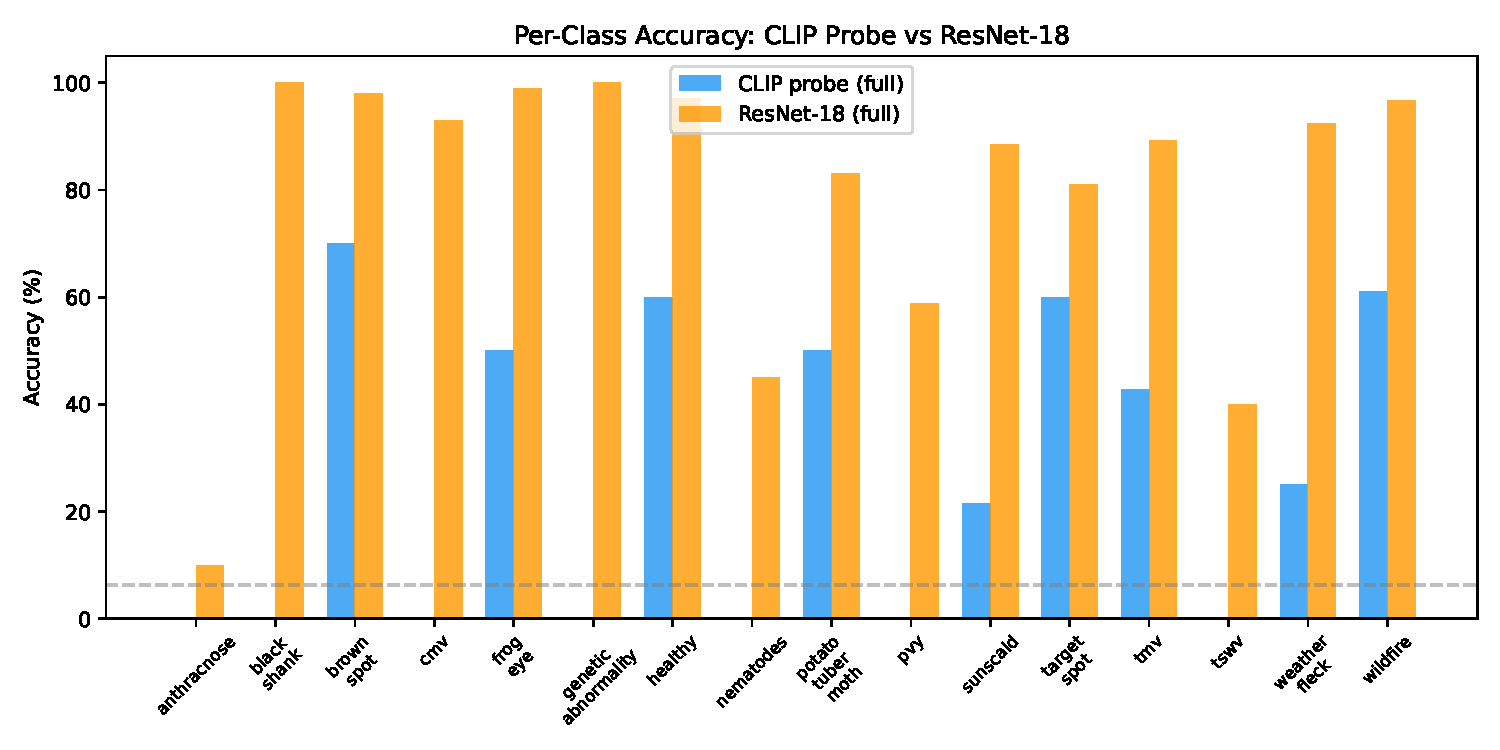
\includegraphics[width=\textwidth]{figures/fig_perclass.pdf}
 \caption{Per-class accuracy: full-data DFN-CLIP linear probe at $C{=}1$ (blue) vs.\ ResNet-18 (orange). DFN-CLIP reaches at least 50\% on 12 of 16 classes, while ResNet-18 reaches at least 50\% on 15 of 16. Dashed line: random chance (6.25\%). The blue/orange scheme is from the Okabe--Ito colorblind-safe palette.}
\label{fig:perclass}
\end{figure}

Figure~\ref{fig:perclass} shows per-class performance.
CLIP's per-class accuracy is highly variable: it is 100\% on a few classes (two of which contain a single test image) and 0\% on the two single-image test classes, strongest on visually clean diseases (healthy, frog eye, brown spot, TMV) and weakest on the confusable ones (nematodes, PVY).
ResNet-18 is stronger overall, reaching at least 50\% on 15 of 16 classes.

Figure~\ref{fig:confusion} presents confusion matrices for both methods.
CLIP probe shows concentrated confusion patterns: most errors involve the model defaulting to a small set of overpredicted classes (e.g., brown\_spot and wildfire are frequently predicted for classes with low per-class accuracy).
ResNet-18's confusion matrix is more diagonal, with errors spread across multiple classes at lower rates.

\begin{figure}[h]
\centering
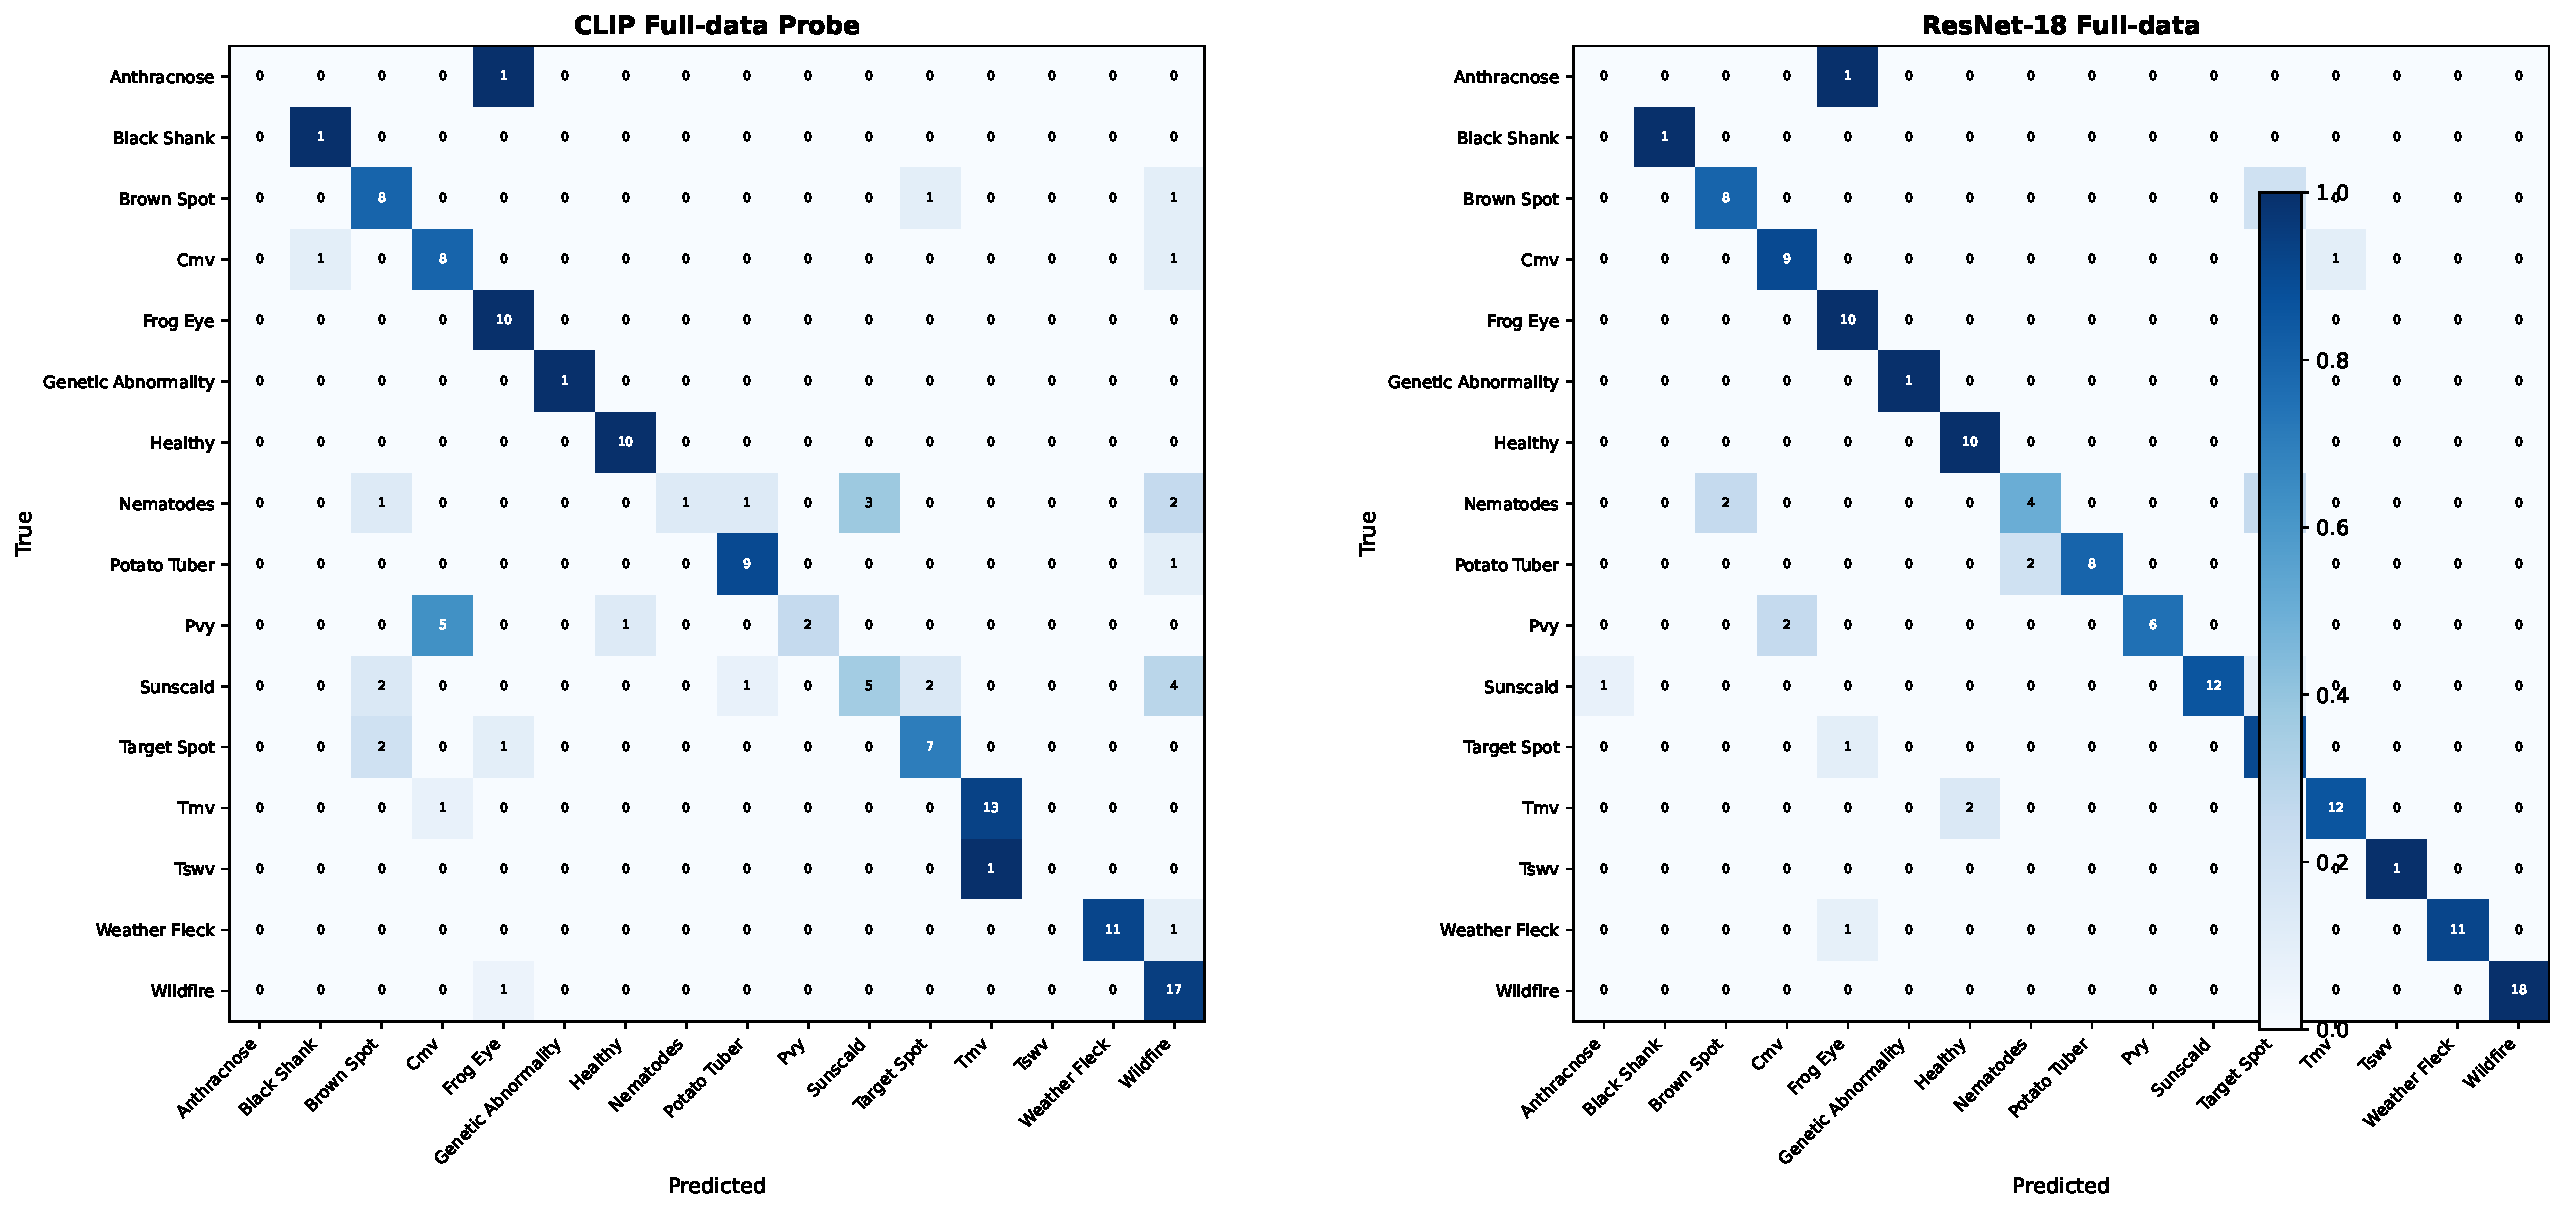
\includegraphics[width=\textwidth]{figures/fig_confusion.pdf}
\caption{Confusion matrices for CLIP full-data linear probe (left) vs.\ ResNet-18 full-data (right) on TPDD test set.}
\label{fig:confusion}
\end{figure}

\subsection{Why Does Generic CLIP Underperform on Fine-Grained Lesions?}
\label{sec:why}

Three complementary analyses characterize how well the frozen CLIP features separate the 16 fine-grained classes, and how much of the classification gap is attributable to the classifier head versus the representation itself.

\textbf{Feature geometry.} Geometry is reported on \emph{both} splits, since the training-split value alone can mislead. In the L2-normalized feature space the mean inter-class centroid distance is smaller than the mean intra-class distance on the training split for both representations. The inter/intra ratio is defined as the mean pairwise distance between class centroids divided by the mean within-class pairwise distance (off-diagonal, i.e., excluding each point's distance to itself), averaged over classes with more than one sample. Under this definition the ratio is 0.62 for the CLIP features and 0.55 for frozen ImageNet-pretrained ResNet-18 features (512-dim, L2-normalized), and on the test split 0.81 for CLIP and 0.79 for ResNet (i.e., within 2pp of each other on the held-out set). A pure-geometry $k$NN(1) classifier on the CLIP features reaches 71.0\%.
The two representations have broadly similar class-separation geometry on both splits: the Fisher discriminant ratio is 0.38 (train) / 0.53 (test) for CLIP and 0.30 (train) / 0.44 (test) for ResNet, and silhouette scores are near zero for both (CLIP $+0.02$ train / $-0.02$ test; ResNet $+0.02$ train / $+0.01$ test). Notably, the CLIP test-split Fisher ratio (0.53) exceeds its training-split value (0.38): the held-out classes are, if anything, more separable in feature space, consistent with the zero-shot failure being attributable to the zero-shot text--image decision rule rather than to the measured feature geometry.
The accuracy difference between the CLIP probe (76.8\%) and the frozen ResNet probe (73.2\%) is therefore not accounted for by a large difference in the measured class-separation geometry.
Figure~\ref{fig:tsne} shows a t-SNE projection of the 138 test-set CLIP features: the 16 classes form overlapping clusters, particularly for the visually confusable fine-grained classes (nematodes, PVY, CMV, sunscald).

\begin{figure}[h]
\centering
\includegraphics[width=0.85\textwidth]{figures/fig_feature_space.pdf}
\caption{t-SNE projection of frozen CLIP features on the 138-image TPDD test set (perplexity=30, max\_iter=1000, random\_state=42). What to look for: tightly separated, well-defined clusters indicate classes the model can distinguish; overlapping clusters (e.g., the visually confusable nematodes/PVY/CMV/sunscald group) indicate classes that share feature space and are hard to separate. This is a qualitative view consistent with the quantitative inter/intra-class geometry analysis above; note that t-SNE geometry on 138 points is not stable across perplexity or random-seed choices and should not be read as quantitative evidence.}
\label{fig:tsne}
\end{figure}

\textbf{Regularization, not representation, explains the residual full-data gap.} As established in Section~\ref{sec:results} (RQ2, Table~\ref{tab:cgrid}), on the \emph{same} frozen CLIP features selecting the probe's regularization on a held-out validation split lifts the default $C{=}1$ probe from 76.8\% to 85.5\%, reaching within $\approx$0.9\,pp of fine-tuned ResNet-18 (86.4\%), while the $k$NN(1) head (71.0\%) and the 256--64 MLP (82.6\%) sit at or below the tuned linear probe and the frozen ResNet-18 features trail at every head (73.2\% linear, 72.5\% MLP); the one tested head that exceeds the tuned linear probe is the exploratory RBF-SVM (87.0\% top-1, 84.8\% balanced), which we report separately as an exploratory within-noise check and do not use as the primary figure. The diagnostic point is that, under the heads tested, the frozen CLIP representation is not the binding constraint on top-1 accuracy; CLIP's remaining consistent disadvantage is on balanced accuracy (the rare fine-grained classes), not on top-1 accuracy.

\textbf{Confusion structure.} The test-set confusion matrix is dominated by a handful of visually confusable fine-grained classes. The most frequent errors are nematodes misread as sunscald (5 of 8, 62\%), Potato virus Y misread as CMV (4 of 8, 50\%), target spot misread as brown spot (2 of 10), and weather fleck and sunscald misread as wildfire (2 of 12 and 2 of 14). These confusions are consistent with distinctions that depend on subtle lesion shape, texture, or symptom context rather than gross appearance.

\textbf{Why the checkpoint and the architecture matter.} The two CLIP checkpoints are the same architecture (ViT-L/14) and differ only in their pretraining data and objective; the split at $K{=}1$ (the LAION-2B probe leads, the DFN-CLIP probe trails) is therefore attributable to pretraining rather than architecture, and the very-low-data regime is the one in which the frozen representation carries most of the classification load and is thus most sensitive to that difference. More generally, CLIP's contrastive image--text objective aligns holistic appearance with coarse natural-language labels, which can privilege gross, object-level cues over the subtle local lesion distinctions (shape, texture, symptom context) that separate the confusable classes above---a plausible reason the fine-grained classes remain the hardest regardless of checkpoint.
\textbf{Scale control.} The frozen CLIP backbone is a 428M-parameter ViT-L/14 whereas the fine-tuned ResNet-18 has 12M parameters---a $\sim$35$\times$ scale gap. Fine-tuning a larger CNN under the identical protocol (ResNet-50, 25.6M, $\sim$2$\times$ ResNet-18 and still $\sim$1/17 of CLIP) raises the fine-tuned-CNN result to $89.6\%\pm2.2$ ($n{=}5$), above ResNet-18 ($86.4\%$) but below fine-tuned CLIP ($94.8$--$96.7\%$). The fine-tuned-CNN result is therefore somewhat scale-dependent (a larger CNN does modestly better), yet the ordering is robust: a compact fine-tuned CNN (ResNet-18/50) reaches the frozen-CLIP-probe level, while giving CLIP the same tuning budget places it on top. The scale asymmetry in the primary frozen-CLIP vs.\ fine-tuned-ResNet-18 comparison thus does not flatter the CNN, and the near-parity is a property of the tested configurations rather than an artifact of an unusually small CNN. Exact values: \texttt{data/resnet50\_full.json}.

Together, these indicate that the representation contains substantial disease-discriminative information (as evidenced by 76--84\% accuracy with supervised heads), but that this information is not aligned with the zero-shot text-space decision geometry and is not optimally accessible to a default linear probe. The pre-specified heads (logistic regression at various $C$, a 256--64 MLP, kNN) all fall at or below fine-tuned ResNet-18 on the primary protocol; the exploratory RBF-SVM head modestly exceeds it ($87.0\%$ vs.\ $86.4\%$, within small-test-set noise). Untested heads (e.g., attention-based pooling, adapters, LoRA) might further change the picture, but they are not tested.

%%%%%%%%%%%%%%%%%%%%%%%%%%%%%%%%%%%%%%%%%%
\section{Discussion}
\label{sec:discussion}

\subsection{Calibration Analysis}

Confidence is miscalibrated in both regimes, but in opposite directions: CLIP is overconfident zero-shot and underconfident under the linear probe.
For zero-shot classification (KG-Symptom), the expected calibration error (ECE) is 0.14, with the model being overconfident across all confidence bins.
Mean confidence of correct predictions (0.32) is slightly higher than that of incorrect ones (0.29), but the gap is small, and the absolute confidence values (0.20--0.45) are modest: CLIP zero-shot is mildly overconfident but does not produce near-certain wrong predictions.

For the full-data linear probe, ECE is 0.46, reflecting the opposite pattern: the logistic regression produces under-confident predictions. Mean confidence of correct predictions (0.31) exceeds that of incorrect ones (0.21), so the probe's confidence ranking is informative even though the absolute values are conservative.
In neither regime are the absolute confidence values calibrated for deployment: they should not be used as decision thresholds without recalibration.

\subsection{Zero-Shot Sits at the Baseline; Features Are Strong}

The core finding is a regime contrast: the identical frozen features that fail zero-shot become competitive with a fine-tuned CNN once given minimal domain data.
CLIP zero-shot shows no detectable improvement over the trivial majority-class baseline on fine-grained lesions (best of 14 templates: 13.0\%, the same as always predicting the most frequent class), indicating that web-scale pretraining does not, on its own, transfer to this domain. This is consistent with the domain-adaptation literature: SCOLD and BioCLIP 2 report that zero-shot competence on fine-grained leaf and biological tasks emerges only after additional domain-specific pretraining, and LP++ shows that a learnable blending head outperforms naive CLIP probing---our result bounds how far off-the-shelf CLIP falls short of that adaptation when none is provided.
With minimal domain training, however, CLIP features become strong: the standard (LAION-2B) variant attains a higher accuracy at $K=1$ (38.5\% vs.\ ResNet-18's 32.1\%; seed-paired, $+6.4$\,pp), the DFN variant trails by 3.7\,pp (28.4\% vs.\ 32.1\%), and at $K=5$--$10$ the fine-tuned ResNet leads both CLIP probes (59.1\%/66.5\% vs.\ 64.7\%/75.2\%).
At $K\geq10$ and with full data, fine-tuned ResNet-18 leads under the default probe (86.4\% vs.\ 76.8\% for both CLIP variants; a gap that selecting $C$ largely closes to 85.5\%).
Crucially, under an identical frozen-backbone protocol the CLIP features lead frozen ResNet-18 by 3.6\,pp (76.8\% vs.\ 73.2\%), and selecting the probe's regularization ($C$) on the \emph{same} frozen CLIP features reaches 85.5\%, within $\approx$0.9\,pp of fine-tuned ResNet-18 (86.4\%) on top-1 accuracy across the 15 training runs (a descriptive gap; no equivalence claim), though the balanced-accuracy gap remains in ResNet's favor (84.3\% vs.\ 77.4\%; Section~\ref{sec:why}).
End-to-end training on domain data still helps, but with minimal domain training CLIP features are a checkpoint-specific, training-light baseline at low data ($K=1$: 28.4--38.5\% vs.\ 32.1\% for ResNet-18), an advantage that is checkpoint-specific and partly a probe-protocol artifact (a frozen ResNet-18 probe scores 34.1\%).

\subsection{Relation to Domain-Specific Vision-Language Models}

Our negative zero-shot result is specific to \emph{off-the-shelf} CLIP and should not be read as a bound on domain-specific vision-language models. SCOLD~\cite{scold2025} (pretrained on $>$186K leaf image--caption pairs) and BioCLIP 2~\cite{bioclip2} (214M organism-image contrastive pretraining) report emergent zero-shot competence on fine-grained leaf and biological tasks that generic CLIP lacks, and LP++~\cite{lpplus} shows a learnable blending head substantially outperforms naive CLIP probing. We did not evaluate any of these in this study (no new experiments), so we do not claim that domain-specific VLMs would also fail at zero-shot. The expected direction is that additional domain pretraining raises the zero-shot baseline above the majority-class level we observe, but the magnitude---and in particular whether it would close the fine-grained gap on the confusable classes---is an open question we leave to future work. Our contribution is therefore the \emph{off-the-shelf} boundary: how far generic CLIP falls short of that domain adaptation when none is provided, and the regime-dependent behavior of its frozen features under minimal domain data.

\subsection{Knowledge-Graph Prompts: No Reliable Benefit Under Present Conditions}

Contrary to the initial hypothesis, KG-augmented prompts did \emph{not} reliably outperform plain caption prompts under the experimental conditions.
On TPDD, the best KG template (KG-Symptom, 13.0\%) ties the plain EN-Photo caption, and the top templates' 95\% confidence intervals all include the 13.0\% majority-class baseline.
On TLD, KG-Symptom (9.5\%) is below the best plain caption (17.7\%), though this comparison is confounded by cross-dataset class mapping uncertainty (TPDD's 16-class KG descriptions mapped to TLD's 10-class vocabulary).
Two important caveats bound this conclusion: first, 7 of 16 TPDD classes lack KG descriptions and use generic fallback text, so the KG templates are a mixture of KG and non-KG prompts and any KG effect is diluted; second, the TLD evaluation relies on a cross-dataset class mapping that may not be semantically precise.
It is therefore not claimed that knowledge-graph prompting is inherently ineffective; rather, the evaluated KG prompting strategy did not demonstrate a benefit under the present class mapping and incomplete KG coverage.

\subsection{Deployment Cost Analysis}

A final, practice-oriented question underlies this section---given a compute budget, which model should a practitioner actually deploy? We answer it here rather than as a separate research question.

For deployment the decisive factor is inference cost rather than training cost, and the compact fine-tuned ResNet-18 is cheaper on both (Table~\ref{tab:cost}). Two scope limits apply to all deployment claims here: the accuracy evidence rests on controlled, close-up leaf imagery (TPDD, TLD), not uncontrolled field imagery, so real-world field accuracy is not measured; and the cost figures in Table~\ref{tab:cost} are measurements on a desktop GPU (NVIDIA RTX 4070 Ti), not on actual edge hardware.
In a typical workflow both models are trained once (in the cloud or on a workstation) and then deployed for inference on lower-cost targets (mobile phones, field laptops, or on-tractor terminals); the comparison below is a relative one (ResNet-18 vs.\ CLIP), not an absolute certification for any particular device.
Under this framing, the relevant trade-offs are inference latency and memory, not training cost: on the measured desktop platform ResNet-18 is $\sim$33$\times$ faster at inference (3{,}900 vs.\ 116 images/s) and uses $\sim$3$\times$ less peak memory (1.1 vs.\ 3.5~GB), making it the more practical choice for resource-constrained inference.
CLIP's advantage is confined to the classifier-training phase: once CLIP features have been extracted, the logistic-regression head can be trained on a CPU, which is useful for a quick research baseline (the feature-extraction step itself still requires the CLIP encoder).

\begin{table}[h]
\centering
\caption{Computational cost comparison.}
\label{tab:cost}
\small
\begin{tabular}{lcc}
\toprule
\textbf{Factor} & \textbf{CLIP Probe} & \textbf{ResNet-18} \\
\midrule
Backbone training & No (frozen) & Yes (30 epochs) \\
Feature extraction & Yes (one-time, GPU) & Within training \\
Head training & Seconds (CPU) & Joint \\
Inference speed (batch 138, FP32) & $\sim$116 imgs/s & $\sim$3{,}900 imgs/s \\
Model size & 1.7 GB (428M params) & 11.6M params ($\sim$45 MB) \\
Peak memory (batch 138) & 3.5 GB & 1.1 GB \\
\midrule
Best accuracy (full, $C$ selected) & 85.5\% (DFN) / 86.2\% (LAION) & 86.4\% \\
\bottomrule
\end{tabular}
\smallskip
{\small Measured 2026-09-10 on a desktop GPU (NVIDIA RTX 4070 Ti, 12~GB); edge-hardware throughput was not measured. Inference throughput and peak memory at batch 138 (3 reps after 2 warmup); ResNet training time = mean of 15 full-data seeds (30 epochs). Exact values and protocol: \texttt{data/full\_provenance.json}.}
\end{table}

For deployment on lower-cost targets (mobile phones, field devices), ResNet-18 is the more practical choice: it is $\sim$33$\times$ faster at inference and uses $\sim$3$\times$ less memory on the measured desktop platform (edge-hardware measurements are not reported).
CLIP's training-phase advantage (the logistic head can be trained on a CPU once features are extracted) is relevant for a quick research baseline; for inference on resource-constrained devices the compact fine-tuned model is preferred.

\subsection{Practical Implications}

For the genuinely low-resource path---no domain data and no domain-specific VLM, as in many smallholder settings---the honest consequence of our findings is that zero-shot off-the-shelf CLIP is not a viable leaf-disorder classifier, and a labeled fine-tuned model (or expert triage) is required; the recommendations below assume at least some domain-labeled data.

\begin{enumerate}
    \item \textbf{Do not rely on CLIP zero-shot for disease diagnosis.} On both datasets the best of 14 templates sits at or below the majority-class baseline (TPDD 13.0\%; TLD 17.7\% vs.\ a 19.0\% baseline). We do not assume a single universal ``operational threshold,'' because it is set by the grower's cost trade-off between a missed infection (a false negative that can spread and reduce yield) and a false alarm (an unnecessary treatment cost or action). In the usual crop-disease case a missed infection costs more than a false alarm, so any defensible threshold sits well above the observed zero-shot accuracy; on that basis zero-shot CLIP fails the test for this use case. Where the cost model is unknown, the safe design is an abstention rule---route uncertain images to an expert or to a calibrated classifier---rather than acting on zero-shot CLIP outputs. No template showed a statistically reliable advantage over the trivial baseline under the test protocol. This zero-shot result is the one that generalizes across the two datasets (RQ3); the CLIP--ResNet comparison cannot be externally validated, because the TLD release provides only a test split.
    \item \textbf{Use frozen CLIP features as a training-light research baseline.} At $K=1$ the standard CLIP variant attains a higher accuracy (38.5\% vs.\ 32.1\% for ResNet-18; seed-paired, $p=0.0003$); at full data both CLIP variants reach 76.8\% under the default probe and 85.5--86.2\% with $C$ selected on a validation split. When a CLIP encoder is already available, the head is cheap to train; for inference on resource-constrained devices prefer the compact fine-tuned model. ``Training-light'' here refers to compute (frozen features, a CPU-trainable head), not to labeling: domain-labeled images are still required, so the practical prerequisite is expert labeling; in that setting CLIP's complementary value is as a weak-label or label-assistant source rather than a labeling-free option.
    \item \textbf{KG-augmented prompts did not help in this setting.} KG-augmented prompts did not improve zero-shot accuracy over plain captions under the evaluated implementation (7 of 16 classes lack KG descriptions, a single English CLIP tokenizer, and a TPDD--TLD class mapping); this does not establish that KG prompting is generally unhelpful, only that the tested configuration showed no benefit.
    \item \textbf{Prefer fine-tuned ResNet-18 when data and GPU are available.} Its clearest advantage is on balanced accuracy (84.3\% vs.\ 77.4\% at the validation-selected $C$), a metric strongly influenced by the four singleton test classes (Table~\ref{tab:perclass}), and it is cheaper to deploy than a CLIP encoder. On top-1 accuracy the full-data gap is small---a validation-regularized CLIP probe within $\approx$0.9\,pp (85.5\% vs.\ 86.4\%; descriptive, not an equivalence claim; Section~\ref{sec:method}). We frame this as a consequence trade-off rather than a raw accuracy ranking: ResNet-18 is the lower-risk, cheaper-to-run option on the rare classes that dominate the balanced-accuracy gap. (The exploratory RBF-SVM head modestly exceeds ResNet-18 at 87.0\%, within small-test-set noise, but is not the pre-specified primary protocol and does not change a deployment choice driven by cost and rare-class robustness.)
    \item \textbf{Treat CLIP confidence with care.} Zero-shot predictions are mildly overconfident (ECE=0.14) while probe predictions are conservative (ECE=0.46); correct predictions have higher mean confidence than incorrect ones in both cases, so the confidence ranking is informative, but absolute thresholds should not be trusted without calibration.
\end{enumerate}

\subsection{Limitations}

(1) Two generic CLIP variants (DFN-CLIP and LAION-2B, both ViT-L/14) are evaluated; the full protocol is additionally replicated cross-crop on tomato (PlantVillage), confirming the regime-by-regime pattern is not tobacco-specific, but generalization to other VLM families (ViT-B/H, SigLIP) and to further crops beyond the two tested (tobacco and tomato) requires further study. Domain-specific VLMs (e.g., BioCLIP 2, SCOLD) and the domain-adapted LP++ probe are not evaluated, and whether such models would lift the zero-shot baseline in this fine-grained setting remains open.
(2) Linear probing plus a CoOp text-prompt control is evaluated; image-branch adapters (LoRA, prompt tuning) may improve CLIP results and merit investigation.
(3) KG-augmented prompts did not reliably help (within noise of plain captions on TPDD, below them on TLD); why domain knowledge in the prompt does not transfer to fine-grained lesions is an open question.
(4) The CNN baseline is scale-limited: we test ResNet-18 (12M) and ResNet-50 (25.6M) but not modern larger CNNs (ConvNeXt, RegNet) or a CNN at CLIP's 428M scale. ResNet-50 already narrows the gap to fine-tuned CLIP ($89.6\%$ vs.\ $94.8$--$96.7\%$), so a scale-matched CNN comparison is not performed---a 400M+ CNN from scratch would overfit on 1{,}295 images, which is precisely why the compact-CNN comparison is the informative one.
(5) The external TLD dataset is a community-contributed collection (Hugging Face, 2024) without a published collection protocol or original dataset paper; its provenance, geographic distribution, and potential duplication with TPDD are not independently verifiable.
(6) LP++ (a learnable image-text knowledge blending linear probe) is cited as prior work but not evaluated; a direct comparison would strengthen the head-capacity analysis.
(7) The full-data comparison uses a logistic probe ($C{=}1$ default; $C$ selected on a 20\% validation split, where the validation top is flat across $C\in\{100,300,1000,3000\}$ (90.0--90.4\%) with the argmax tied at $C\in\{300,3000\}$; the lower-complexity $C{=}300$ is reported, reaching 85.5\%) and a minimal CoOp control (4 tokens, 10 epochs). The validation-selected probe on frozen CLIP features reaches 85.5\% (vs.\ ResNet-18's 86.4\%), a $\approx$0.9\,pp difference across the 15 ResNet training runs (a descriptive top-1 near-parity, no equivalence claim; 15-seed CI $\approx[-0.1,\,+2.0]$pp; the balanced-accuracy gap remains in ResNet's favor) but is \emph{not} resolvable at the per-image level (per-image SE$\approx$3.4pp). The full-data CLIP numbers use a single clean, deterministic feature-extraction protocol (un-augmented evaluation transform), which is verified to be reproducible across independent runs (byte-identical features and test accuracy); stronger image-branch adapters (LoRA, prompt tuning) are not tested, so the CLIP numbers remain a conservative estimate of what is achievable with this representation. (CoOp is now tested at its full 16-token/20-epoch recipe as well as a minimal 4-token configuration; both are reported in Section~\ref{sec:results} and collapse to near chance, so CoOp is not a rescue path here.)
(8) Field generalization. All accuracy evidence is on controlled, close-up leaf imagery (TPDD, TLD); how either model performs under uncontrolled field conditions---variable background, lighting, and disease stage---is an open question we do not address, and the deployment recommendations in Section~\ref{sec:discussion} should not be read as field-condition performance claims.
(9) The fine-tuned-CLIP fairness control (96.7\% / 94.8\% full-data) fine-tunes the image encoder plus a linear head on image labels under a single matched budget; it does not use the full CLIP image--text objective, image-branch adapters (LoRA), or a few-shot fine-tuning sweep, so it is a tuning-budget check confirming the frozen-probe comparison is conservative, not an estimate of CLIP's full fine-tuning ceiling.

%%%%%%%%%%%%%%%%%%%%%%%%%%%%%%%%%%%%%%%%%%
\section{Conclusions}
\label{sec:conclusion}

Generic vision-language models (two CLIP variants) were systematically evaluated for fine-grained leaf-disease classification across three datasets (tobacco TPDD and TLD; tomato PlantVillage), 14 prompt templates, and several training regimes, with bootstrap confidence intervals, two-sample and one-sample $t$-tests, and multi-seed comparisons ($n=15$ seeds).
The key findings are:
(1) Zero-shot CLIP shows no detectable improvement over the trivial majority-class baseline on both datasets (TPDD: best of 14 templates 13.0\% = the 13.0\% baseline; TLD: 17.7\% vs.\ a 19.0\% baseline); no template showed a statistically reliable advantage over the majority-class baseline under the test protocol.
(2) With minimal domain training, the standard CLIP variant (LAION-2B) attains a higher accuracy than ResNet-18 at $K{=}1$ (38.5\% vs.\ 32.1\%; seed-paired, $p=0.0003$) while the DFN-CLIP variant trails at a borderline level (28.4\% vs.\ 32.1\%; $p=0.064$)---the only statistically significant CLIP advantage is therefore checkpoint-specific; at full data both CLIP variants reach 76.8\% under the default probe and 85.5--86.2\% with $C$ selected.
(3) The comparison is regime-dependent. At $K{=}1$ the LAION-2B CLIP probe attains a higher accuracy than fine-tuned ResNet-18 (38.5\% vs.\ 32.1\%; seed-paired support sets, $p=0.0003$) while the DFN-CLIP variant trails by 3.7\,pp, and at $K{=}5$--$10$ the fine-tuned ResNet leads both CLIP probes. At full data a validation-regularized CLIP probe reaches 85.5\%, within $\approx$0.9\,pp of fine-tuned ResNet-18 (86.4\%) on top-1 across the 15 training runs (a descriptive gap, not an equivalence claim; the default un-regularized probe trails at 76.8\%), a single-dataset observation since the external TLD set provides no training split for replication; under 5-fold cross-validation over the training pool, fine-tuned ResNet-18 holds a small, sign-stable edge over the frozen CLIP probe ($87.8\%$ vs.\ $92.1\%$, $-4.3\,\text{pp}\pm1.8$, all five folds), so the full-data result is a close, split-dependent comparison with a modest CNN advantage rather than a systematic CLIP win. On balanced accuracy ResNet-18 shows higher aggregate class-balanced performance (84.3\% vs.\ 77.4\%), a difference driven mainly by a single $n{=}1$ test class (removing it collapses the 6.9\,pp gap to 0.6\,pp) and one mid-frequency class; this is not interpreted as a general superiority for rare classes beyond this test split. (All full-data CLIP numbers are deterministic: clean un-augmented features plus logistic regression on fixed features, verified byte-identical across two independent runs.)
(4) The regime-by-regime pattern is not tobacco-specific: replicated in full on a second crop (tomato, PlantVillage, 18{,}160 images) under the identical protocol, zero-shot CLIP again sits at the majority baseline (33.4\% vs.\ 29.5\%), the frozen CLIP probe is competitive at $K{=}1$ (44.7\% vs.\ 40.4\%) with fine-tuned ResNet-18 leading at $K{=}5$--$10$ (73.6--84.4\%), and full-data near-parity holds with a small, sign-stable CNN edge under 5-fold CV (98.0\% vs.\ 99.5\%, $-1.6\,\text{pp}$, all five folds).
(5) CLIP zero-shot predictions are mildly overconfident (ECE=0.14) while probe predictions are conservative (ECE=0.46); in both cases the confidence ranking is informative even though absolute thresholds are not.

For \emph{off-the-shelf} CLIP specifically---domain-specific VLMs such as SCOLD and BioCLIP 2 are not evaluated here and may behave differently (Section~\ref{sec:discussion})---we recommend that practitioners treat zero-shot CLIP (and KG-augmented prompts) as inadequate for fine-grained tobacco-lesion diagnosis, use frozen-CLIP features with a well-chosen head as a training-light research baseline at low data (the $K{=}1$ advantage is checkpoint-specific), prefer fine-tuned ResNet-18 when data and GPU are available, and verify calibration before any operational deployment.

%%%%%%%%%%%%%%%%%%%%%%%%%%%%%%%%%%%%%%
\section*{Appendix A: Full-Data Protocol and Reproducibility}
\label{appx:protocol}

All full-data CLIP and frozen-ResNet numbers in the paper come from a single clean, deterministic feature-extraction protocol (Section~\ref{sec:why}); there is no protocol-level ambiguity in the reported full-data values. Concretely, features are extracted with the deterministic evaluation transform (resize + center-crop + normalize; no stochastic augmentation), so the frozen features---and hence every full-data number---are identical across runs. This is verified by running the full pipeline twice independently and obtaining byte-identical features and test accuracy. An earlier full-data iteration inadvertently applied the stochastic training transform to the frozen feature extraction, making those features run-dependent; the canonical protocol above corrects that. The CoOp control and the few-shot probe were unaffected by that bug: CoOp uses the clean evaluation transform on both support and test, and the few-shot probe augments only its small support set (standard few-shot practice) while extracting the test set with the clean evaluation transform. Under this single protocol the full-data results are: frozen DFN-CLIP probe $C{=}1$ 76.8\%, validation-selected $C{=}300$ 85.5\% (and 86.2\% for the LAION-2B checkpoint), 256--64 MLP 82.6\%, $k$NN(1) 71.0\%; frozen ResNet-18 features 73.2\% (linear) / 72.5\% (MLP); fine-tuned ResNet-18 86.4\% $\pm$ 1.9\% ($n{=}15$ seeds, the only stochastic side of the comparison). Balanced accuracy (16 classes, 4 of which are single-image test classes): 68.3\% (CLIP $C{=}1$), 77.4\% (CLIP $C{=}300$), 64.9\% (frozen ResNet linear), 84.3\% (fine-tuned ResNet).

%%%%%%%%%%%%%%%%%%%%%%%%%%%%%%%%%%%%%%%%%%
\authorcontributions{Conceptualization, L.L.; methodology, L.L.; software, L.L.; validation, L.L.; formal analysis, L.L.; investigation, L.L.; resources, L.L.; data curation, L.L.; writing--original draft, L.L.; writing--review \& editing, L.L.; visualization, L.L.}
\funding{This research received no external funding.}
\dataavailability{The code and data supporting the findings of this study are available in the project repository; the repository URL will be inserted upon acceptance.}
\conflictsofinterest{The author declares no conflicts of interest.}

\section*{Abbreviations}
The following abbreviations are used in this manuscript:
\par
\begin{tabular}{@{}l p{0.78\textwidth}@{}}
CLIP & Contrastive Language-Image Pretraining \\
ViT & Vision Transformer \\
TPDD & Tobacco Plant Disease Dataset \\
TLD & Tobacco Leaf Diseases dataset \\
KG & Knowledge Graph \\
CoOp & Context Optimization \\
ECE & Expected Calibration Error \\
PVY & Potato virus Y \\
CMV & Cucumber mosaic virus \\
TMV & Tobacco mosaic virus \\
TSWV & Tomato spotted wilt virus \\
CNN & Convolutional neural network \\
LR & Logistic regression \\
MLP & Multilayer perceptron \\
\end{tabular}

\vspace{6pt}

\reftitle{References}

\begin{thebibliography}{99}

\bibitem{radford2021learning}
Radford, A.; Kim, J.W.; Hallacy, C.; Ramesh, A.; Goh, G.; Agarwal, S.; Sastry, G.; Askell, A.; Mishkin, P.; Clark, J.; et al.
Learning Transferable Visual Models From Natural Language Supervision.
In \emph{Proceedings of ICML}, 2021.

 \bibitem{pdclip2026}
 Xie, P.; Li, X.; He, W.; Meadows, I.; Xiang, L.
 PD-CLIP: A contrastive language-image pre-training framework for zero-shot fine-grained plant disease diagnosis.
 \emph{Artif. Intell. Agric.} 2026.
 https://doi.org/10.1016/j.aiia.2026.08.012

\bibitem{huang2021gloria}
Huang, S.-C.; Shen, L.; Lungren, M.P.; Yeung, S.
GLoRIA: A Multimodal Global-Local Representation Learning Framework for Label-Efficient Medical Image Recognition.
In \emph{Proceedings of ICCV}, 2021.
https://doi.org/10.1109/iccv48922.2021.00391

\bibitem{liu2024remoteclip}
Liu, F.; Chen, D.; Guan, Z.; Zhou, X.; Zhu, J.; Ye, Q.; Fu, L.; Zhou, J.
RemoteCLIP: A Vision Language Foundation Model for Remote Sensing.
\emph{IEEE Trans. Geosci. Remote Sens.} 2024.
https://doi.org/10.1109/tgrs.2024.3390838

\bibitem{scold2025}
Nguyen, K.Q.; Le, L.T.T.; Quach, L.-D.
A Vision-Language Foundation Model for Leaf Disease Identification.
\emph{Expert Syst. Appl.} 2026.
https://doi.org/10.1016/j.eswa.2025.130084

\bibitem{bioclip2}
Gu, J.; Stevens, S.; Campolongo, E.; Thompson, M.; Zhang, N.; Wu, J.; Kopanev, A.; Mai, Z.; White, A.; Balhoff, J.; et al.
BioCLIP 2: Emergent Properties from Scaling Hierarchical Contrastive Learning.
In \emph{Advances in Neural Information Processing Systems (NeurIPS)}, 2025.
https://doi.org/10.52202/085713-3436

\bibitem{dinov2}
Oquab, M.; Darcet, T.; Moutakanni, T.; et al.
DINOv2: Learning Robust Visual Features without Supervision.
\emph{Transactions on Machine Learning Research (TMLR)}, 2024.
https://arxiv.org/abs/2304.07193

\bibitem{lpplus}
Huang, Y.; Shakeri, F.; Dolz, J.; Boudiaf, M.; Bahig, H.; Ben Ayed, I.
LP++: A Surprisingly Strong Linear Probe for Few-Shot CLIP.
In \emph{Proceedings of CVPR}, 2024.
https://doi.org/10.1109/cvpr52733.2024.02244

\bibitem{zhai2023sigmoid}
Zhai, X.; Mustafa, B.; Kolesnikov, A.; Beyer, L.
Sigmoid Loss for Language Image Pre-Training.
In \emph{Proceedings of ICCV}, 2023.
https://doi.org/10.1109/iccv51070.2023.01100

\bibitem{cherti2023reproducible}
Cherti, M.; Beaumont, R.; Wightman, R.; Wortsman, M.; Ilharco, G.; Gordon, C.; Schuhmann, C.; Schmidt, L.; Jitsev, J.
Reproducible Scaling Laws for Contrastive Language-Image Learning.
In \emph{Proceedings of CVPR}, 2023.
https://doi.org/10.1109/cvpr52729.2023.00276

\bibitem{deng2009imagenet}
Deng, J.; Dong, W.; Socher, R.; Li, L.-J.; Li, K.; Fei-Fei, L.
ImageNet: A Large-Scale Hierarchical Image Database.
In \emph{Proceedings of CVPR}, 2009.
https://doi.org/10.1109/cvpr.2009.5206848

\bibitem{stevens2024bioclip}
Stevens, S.; Wu, J.; Thompson, M.J.; Campolongo, E.G.; Song, C.H.; Carlyn, D.E.; Dong, L.; Dahdul, W.M.; Stewart, C.; Berger-Wolf, T.; et al.
BioCLIP: A Vision Foundation Model for the Tree of Life.
In \emph{Proceedings of CVPR}, 2024.
https://doi.org/10.1109/cvpr52733.2024.01836

\bibitem{shinoda2025agrobench}
Shinoda, R.; Inoue, N.; Kataoka, H.; Onishi, M.; Ushiku, Y.
AgroBench: Vision-Language Model Benchmark in Agriculture.
In \emph{Proceedings of ICCV}, 2025, 7634--7644.
https://doi.org/10.1109/iccv51701.2025.00716

\bibitem{zhou2022learning}
Zhou, K.; Yang, J.; Loy, C.C.; Liu, Z.
Learning to Prompt for Vision-Language Models.
\emph{Int. J. Comput. Vis.} 2022, 130, 2337--2348.
https://doi.org/10.1007/s11263-022-01653-1

\bibitem{liu2025finegrained}
Liu, Y.; Deng, Y.; Liu, A.; Liu, Y.; Li, S.
Fine-Grained Multi-Modal Prompt Learning for Vision-Language Models.
\emph{Neurocomputing} 2025, 636, 130028.
https://doi.org/10.1016/j.neucom.2025.130028

\bibitem{cropdpkg2025}
Yan, R.; An, P.; Meng, X.; Li, Y.; Li, D.; Xu, F.; Dang, D.
A Knowledge Graph for Crop Diseases and Pests in China.
\emph{Scientific Data} 2025, 12, 222.
https://doi.org/10.1038/s41597-025-04492-0

\bibitem{argueso2020fewshot}
Argüeso, D.; Picon, A.; Irusta, U.; Medela, A.; San-Emeterio, M.G.; Bereciartua, A.; Alvarez-Gila, A.
Few-Shot Learning Approach for Plant Disease Classification Using Images Taken in the Field.
\emph{Computers and Electronics in Agriculture} 2020, 175, 105542.
https://doi.org/10.1016/j.compag.2020.105542

\bibitem{liang2021cotton}
Liang, X.
Few-Shot Cotton Leaf Spots Disease Classification Based on Metric Learning.
\emph{Plant Methods} 2021, 17, 114.
https://doi.org/10.1186/s13007-021-00813-7

\bibitem{plantvillage2016}
Mohanty, S.P.; Hughes, D.P.; Salathé, D.
Using Deep Learning for Image-Based Plant Disease Detection.
\emph{Front. Plant Sci.} 2016, 7, 1419.
https://doi.org/10.3389/fpls.2016.01419

\bibitem{plantvillage_mendeley}
Plant Leaf Diseases Dataset (without augmentation); tomato subset.
\emph{Mendeley Data}, 2024.
https://doi.org/10.17632/tywbtsjrjv.1

\bibitem{lin2022tpdd}
Lin, H.; Tse, R.; Tang, S.-K.; Qiang, Z.; Ou, J.; Pau, G.
Tobacco Plant Disease Dataset.
In \emph{Proceedings of the 14th International Conference on Digital Image Processing (ICDIP)}, 2022, 89.
https://doi.org/10.1117/12.2644288

\bibitem{tld}
Joker5800.
Tobacco\_Leaf\_Diseases.
\emph{Hugging Face Datasets}, 2024.
Available online: \url{https://huggingface.co/datasets/Joker5800/Tobacco_Leaf_Diseases}.

\bibitem{fang2023data}
Fang, A.; Jose, A.M.; Jain, A.; Schmidt, L.; Toshev, A.; Shankar, V.
Data Filtering Networks.
\emph{arXiv preprint} arXiv:2309.17425, 2023.

\bibitem{he2016deep}
He, K.; Zhang, X.; Ren, S.; Sun, J.
Deep Residual Learning for Image Recognition.
In \emph{Proceedings of CVPR}, 2016.
https://doi.org/10.1109/cvpr.2016.90

\end{thebibliography}

%%%%%%%%%%%%%%%%%%%%%%%%%%%%%%%%%%%%%%%%%%
\end{document}
